\documentclass[11pt,a4paper]{article}
\usepackage{amsmath,amssymb,unicode-math,lmodern}
\defaultfontfeatures{Ligatures=TeX}
\setmainfont[BoldFont=texgyrepagella-bold.otf,ItalicFont=texgyrepagella-italic.otf,BoldItalicFont=texgyrepagella-bolditalic.otf]{texgyrepagella-regular.otf}
\setmonofont[BoldFont=lmmonolt10-bold.otf]{lmmono10-regular.otf}
\setmathfont{texgyrepagella-math.otf}
\usepackage[margin=25mm,headheight=14pt,headsep=7mm]{geometry}
\usepackage{mathtools,booktabs,array,graphicx,xcolor,fancyhdr,needspace}
\newcolumntype{P}[1]{>{\raggedright\arraybackslash}p{#1}}
\usepackage[colorlinks=true,linkcolor=blue!40!black,citecolor=blue!40!black,urlcolor=blue!40!black]{hyperref}
\pagestyle{fancy}\fancyhf{}\lhead{\small Paired driving and exterior identifiability}\rhead{\small Paper II: draft v0.1}\cfoot{\thepage}
\setlength{\parskip}{4pt}\setlength{\parindent}{1.2em}\setlength{\emergencystretch}{2em}\raggedbottom
\newtheorem{theorem}{Theorem}[section]
\newtheorem{proposition}[theorem]{Proposition}
\newtheorem{corollary}[theorem]{Corollary}
\newtheorem{definition}[theorem]{Definition}
\newtheorem{remark}[theorem]{Remark}
\newenvironment{proof}{\par\noindent\textit{Proof.}\ }{\hfill$\square$\par}
\AddToHook{env/theorem/before}{\Needspace{7\baselineskip}}
\AddToHook{env/proposition/before}{\Needspace{6\baselineskip}}
\AddToHook{cmd/subsection/before}{\Needspace{7\baselineskip}}
\AddToHook{cmd/section/before}{\Needspace{10\baselineskip}}
\newcommand{\R}{\mathbb R}\newcommand{\C}{\mathbb C}
\newcommand{\norm}[1]{\lVert#1\rVert}\newcommand{\sinc}{\operatorname{sinc}}
\newcommand{\diag}{\operatorname{diag}}\newcommand{\rank}{\operatorname{rank}}
\newcommand{\ii}{\mathrm i}\newcommand{\dd}{\,\mathrm d}
\newcommand{\tr}{^{\mathrm T}}\newcommand{\ez}{e_z}\newcommand{\tf}{t_{\mathrm f}}
\newcommand{\tref}{t_{\mathrm{ref}}}\newcommand{\F}{\mathcal F}\newcommand{\Jflux}{\mathcal J}
\hypersetup{pdftitle={Paired Driving and Exterior Identifiability on a Conditional Periodic Carrier},pdfauthor={Hilmir Frimann Halldorsson},pdfsubject={Paper II; draft v0.1; conditional mathematical comparison}}
\begin{document}
\begin{center}
{\LARGE\bfseries Paired Driving and Exterior Identifiability\par on a Conditional Periodic Carrier\par}
\vspace{5mm}{\large Hilmir Fr\'imann Halld\'orsson}\par
\vspace{3mm}19 October 2026\quad Paper II\quad Draft v0.1
\end{center}
\begin{abstract}
We connect the paired-gap geometry of the folded Tri-Octagon to an explicitly adopted periodic carrier and passive exterior observation rule. Two distributed tent sources act at the actual non-antipodal contacts of one offset vertical circle. We prove well-posedness, a signed source-work identity, geometry-dependent spectral coupling, and the limits imposed by a persistent mean and undamped resonances. A circular symmetry reduction gives exact singular values for the first-harmonic exterior map. Every equatorial scalar array is blind to travelling direction, even when a shifted standing wave has the same storage and scalar record. Off-height phase measurements or calibrated directional channels resolve this ambiguity within a stated delay range. Starting from rest, a common one-circuit pulse produces a mean plus standing harmonic and zero integrated directional bias at all times. For general finite paired histories we derive the temporal cross-phase criterion; the specified quarter-period lag gives a strong but impure harmonic bias whose total-storage fraction is much smaller when the mean is retained. Source-defined macro and chiral readouts are then compared through an explicit symbolic sample-and-hold convention. The resulting distinctions concern conditional state generation and identification, without identifying model storage with native physical energy. Full proofs, inherited error-qualified reception data and static figures accompany the construction.
\end{abstract}
\tableofcontents
\clearpage
\section{Question, assumptions and inherited geometry}\label{sec:foundations}
Hilmir Fr\'imann Halld\'orsson's geometric proposal places a transverse local loop through paired upper and lower measurement regions of the folded Tri-Octagon and surrounds the central module with complete smaller copies. His subsequent height and radius comparisons ask whether position changes what those copies can receive. Paper I establishes the geometry and distinguishes it from an observation law.~\cite{PaperI} The present paper supplies a precise conditional source-to-observation construction using the already defined C1 carrier and C6 reception map.~\cite{SRG05,SRG06} The question is what paired inputs generate, and which exterior records distinguish the result.

The development follows the author's sustained human--AI mathematical collaboration. The paired geometry and multi-ring questions motivate the analysis; the particular carrier law, reception kernel and pulse calibrations are stated comparison choices. Mathematical usefulness for computation need not await a physical realization of the carrier. Conversely, a useful formula does not establish computational advantage or a natural mechanism. We keep this distinction at the level of definitions and conclusions, while giving the conditional mathematics in full.

There are three stages of evidence. Geometric and native-readout definitions are inherited from Paper I and its source snapshots. C1 and C6 are explicit adoptions, not deduced from those definitions. The finite pulse and timing controls are prescribed tests of the adopted system; their generated states and identification results are deductions. The numerical matrices reported below are retained SRG-06--08 results, with their original error qualifications.~\cite{SRG07,SRG08,Reviews} No new reception quadrature or trajectory is needed for this consolidation.

\subsection{One circle, actual contacts and complete observers}
Use the width-one folded shell of Paper I, with origin $O=(0,\sqrt3/6,0)$, $u=(0,1,0)$, $v=\ez\times u=(-1,0,0)$ and $\ez=(0,0,1)$. Define
\begin{equation}\label{eq:geometry}
 K=\frac{\sqrt3}{12}+\frac{\sqrt6}{4},\qquad
 a=\frac{K}{1+\sqrt3/2},\qquad R=\frac{\sqrt7a}{2},\qquad L=2\pi R.
\end{equation}
The selected local centreline, with its fixed orientation, is
\begin{equation}\label{eq:circle}
 \Gamma(s)=B_0+R(\cos\chi\,u+\sin\chi\,\ez),\quad
 B_0=O+Ku,\quad \chi=s/R\pmod{2\pi},\quad
 \hat t=-\sin\chi\,u+\cos\chi\,\ez.
\end{equation}
It is a vertical offset circle. The central shell remains the folded annulus; the circle is an additional conditional construction, not a new material edge or a join of the boundary rims. Its two contacts and signed readout normals are
\begin{equation}\label{eq:contacts}
 P_\pm=O+au\pm a\ez,\qquad n_\pm=(2u\pm\sqrt3\ez)/\sqrt7.
\end{equation}
Write $\theta=\arctan(2/\sqrt3)$ and $\eta=R\theta$. The correct quadrants give
\begin{equation}\label{eq:arcs}
 s_+=L/2-\eta,\quad s_-=L/2+\eta,\qquad
 \ell_{\rm short}=2\eta,\quad\ell_{\rm long}=L-2\eta.
\end{equation}
Indeed $\cos\chi_\pm=-\sqrt{3/7}$ and $\sin\chi_\pm=\pm2/\sqrt7$, so the contact tangents are $-n_+$ and $+n_-$. These facts do not insert a sign in the later source law. The arcs are approximately $0.9195560877$ and $2.4510718473$, with $R=0.5364520972$ and $L=3.3706279350$. The contacts are neither antipodal nor snapped to a twelve-site grid.

For observer index $k=0,\ldots,11$, let $\psi_k=\pi/2+k\pi/6$, $e_r=(\cos\psi_k,\sin\psi_k,0)$ and $e_\psi=(-\sin\psi_k,\cos\psi_k,0)$. The inherited centres, frames and full miniature vertices are
\begin{equation}\label{eq:observers}
 X_{mk}=O+\rho_m e_r+h_m\ez,\qquad B_k=[e_r,\ez,-e_\psi],\qquad
 P\longmapsto X_{mk}+\tfrac14 B_k(P-O).
\end{equation}
Every original vertex and face is retained under this map. H uses $\rho_m=3$ and $h_m/a=2,1,0,-1,-2$; R1,R2,R3 use $\rho_m=2,3,4$ at $h_m=0$. The 96 labels describe 84 distinct sites, because H0 and R2 coincide in both centre and frame. A combined height-by-radius product is not instantiated. The quarter-turn fixes the frame; centre sampling below does not turn miniature surface area into a receiving area.

\begin{figure}[htbp]\centering
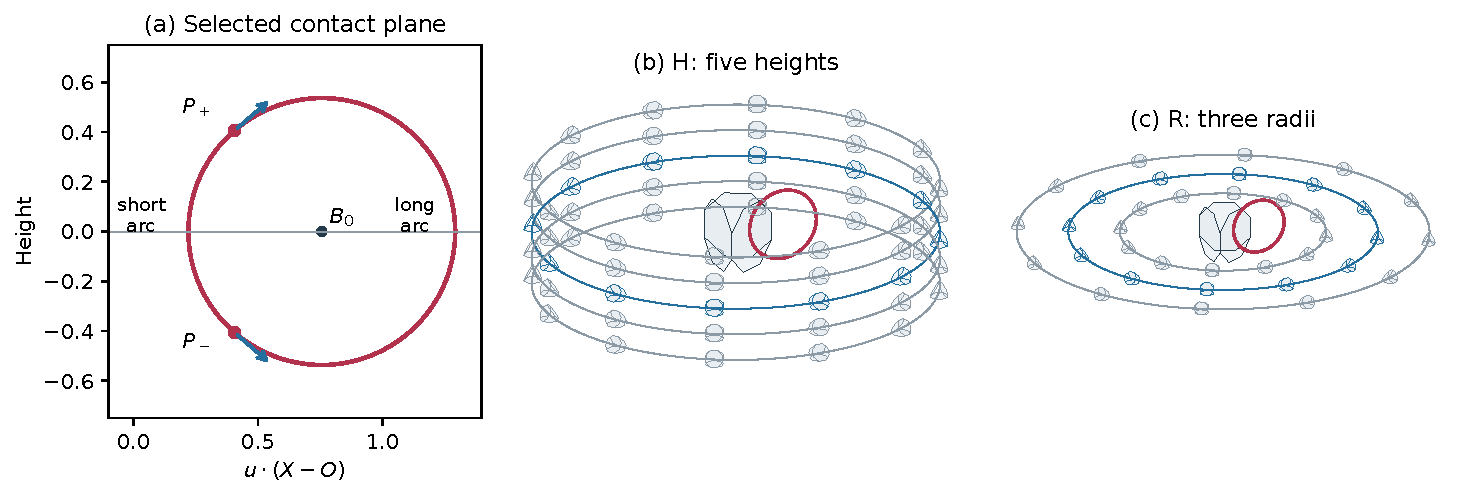
\includegraphics[width=\textwidth]{figures/geometry.pdf}
\caption{Inherited geometry and conditional carrier. The median view shows the actual contacts and unequal arcs of $\Gamma_0$; the paired normals are readout covectors. The separate H/R views retain all complete quarter-scaled modules. Their placement rings are reference curves, not carriers. Blue marks H0/R2, the same twelve sites. No line joining a source to a receiver represents a material connection.}\label{fig:geometry}
\end{figure}

\subsection{Typed input chain and the missing component}\label{sec:typed}
Let $\Omega\in\C^3$ be the native state. The separately defined readouts include
\begin{equation}\label{eq:readouts}
 I=\norm{\Omega}^2,\quad C=\Re\Omega\times\Im\Omega,\quad
 M=z(\cos\vartheta_c,\sin\vartheta_c,1),
\end{equation}
where the staged scalar is
\begin{equation}\label{eq:staged}
 z=\lambda_{vp}\frac{\sqrt I}{1+\sqrt I}
 \cos[3(\vartheta_c-\vartheta_{\rm lock})]e^{-\gamma t_{\rm clock}}.
\end{equation}
The integer clock $q$ supplies $\vartheta_c=2\pi(q\bmod N)/N$. The source also defines the blend $T_{\rm blend}=\alpha M+\beta C$; it is not a third independent state. These formulas are numerical readouts and are not an ambient field law.~\cite{Native}

For one named family $v_{\rm in}=M$ or $C$, fix the inherited dictionary $A=\lambda_gR_z(\delta_g)$. The chain is
\begin{equation}\label{eq:sourcechain}
 \Omega,\text{ clock/configuration}\longmapsto v_{\rm in}
 \longmapsto W=Av_{\rm in}\longmapsto q_\pm=n_\pm\tr W
 \longmapsto f_\pm=\kappa_{\rm in}q_\pm.
\end{equation}
The positive common gain $\kappa_{\rm in}$ is an adopted conversion of data units to source strength. It is not an energy efficiency. Writing $W=W_ru+W_av+W_z\ez$, define
\begin{equation}\label{eq:sectors}
 f_s=\tfrac12(f_++f_-)=\frac{2\kappa_{\rm in}}{\sqrt7}W_r,
 \qquad f_a=\tfrac12(f_+-f_-)=\frac{\sqrt3\kappa_{\rm in}}{\sqrt7}W_z.
\end{equation}
The kernel of this pair projection is exactly $\operatorname{span}(v)$. Equal projected histories and equal carrier preparation give equal downstream states and records by uniqueness. An added observer cannot recover $W_a$ or a native cubic invariant $J$ lost upstream. At fixed readout clock, $M$ has only one real scalar freedom, even though the abstract two-port calibration has two input coefficients.

\subsection{Conventions and dimensions}\label{sec:units}
The width normalization is geometric. Multiplying all coordinates by a length unit restores dimensional lengths; no SI length or time is selected. We denote dimensions by $\mathrm L,\mathrm T,\mathrm U,\mathrm Q$ to avoid confusing them with the circumference $L$ or the pulse duration $T$.
\begin{table}[htbp]\centering\small
\begin{tabular}{P{.29\textwidth}P{.35\textwidth}P{.23\textwidth}}\toprule
Symbol & Meaning & Dimension\\\midrule
$s,R,L,\epsilon,d$ & Arclength, radius, width, distance & $\mathrm L$\\
$t,c,c_e$ & Analysis time; two independent speeds & $\mathrm T$; $\mathrm L/\mathrm T$\\
$p,r$ & Real carrier variables & $\mathrm U$\\
$b_\pm; f_\pm$ & Normalized profiles; source strengths & $\mathrm L^{-1}$; $\mathrm U\mathrm L/\mathrm T$\\
$q_\pm;\kappa_{\rm in}$ & Input data; common conversion & $\mathrm Q$; $\mathrm U\mathrm L/(\mathrm T\mathrm Q)$\\
$e;E$ & Storage density; total storage & $\mathrm U^2$; $\mathrm U^2\mathrm L$\\
$j;f_\pm y_\pm$ & Local oriented flux; source power & $\mathrm U^2\mathrm L/\mathrm T$\\
$\Jflux=\int j\dd s$ & Spatially integrated oriented flux & $\mathrm U^2\mathrm L^2/\mathrm T$\\
$U,V,Y$ & Scalar, vector, local exterior record & $\mathrm U$\\
$g_o$ & Common exterior calibration & Dimensionless\\\bottomrule
\end{tabular}
\caption{Model dimensions. In particular, $\Jflux$ is not power through a section.}\label{tab:units}
\end{table}

Spatial Fourier coefficients use $L^{-1}\int_0^L f(s)e^{-\ii ns/R}\dd s$. Temporal phasors use $e^{+\ii\omega t}$, and finite transforms use $\int f(t)e^{+\ii\omega t}\dd t$. Thus an exterior delay contributes $e^{-\ii\omega d/c_e}$. A directional amplitude subscript denotes propagation, not a source-port label. We use normalized characteristics $w_\sigma=(p+\sigma r)/\sqrt2$ throughout; the unnormalized convention in SRG-08 is $\widetilde w_\sigma=\sqrt2w_\sigma=p+\sigma r$.

The native iteration index, the readout clock $(q,t_{\rm clock})$, carrier time $t$, arclength $s$ and observer index $k$ are independent variables. Later $T=L/c$ is a prescribed pulse scale, not $T_{\rm blend}$. Reception moments are $H,S_m,C_m$; $C_m$ is never the native readout $C$. The frame $B_k$, tent factor $B_n$ and centre $B_0$ have distinct subscripts and types.

\begin{figure}[htbp]\centering
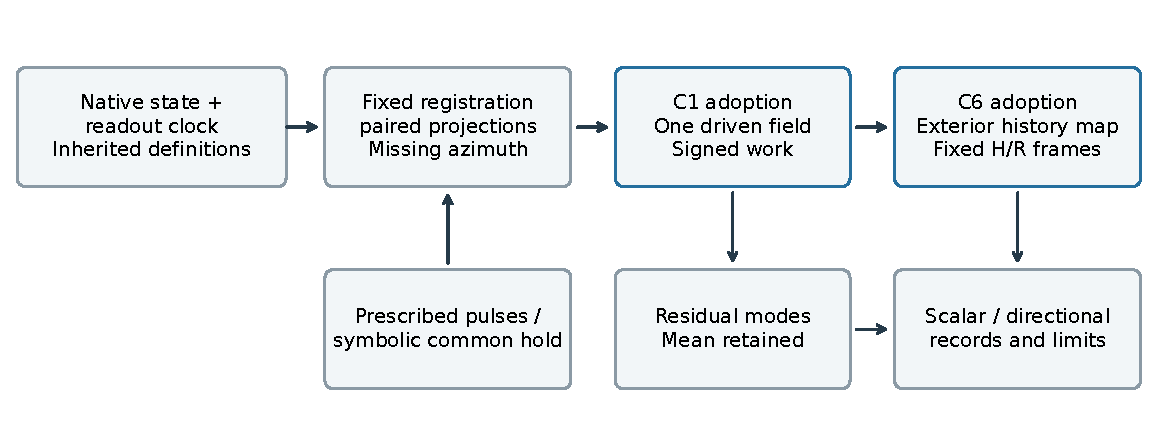
\includegraphics[width=\textwidth]{figures/dependencies.pdf}
\caption{Dependency and information boundaries. Solid boxes are defined objects; arrows state explicit maps. C1 and C6 are separate adoptions. The sample-and-hold bridge in Section~\ref{sec:native} is conditional and uses symbolic cadence. Observer duplication adds records without adding a state or modifying source work.}\label{fig:dependencies}
\end{figure}

\section{A shared periodic carrier and its source account}\label{sec:carrier}
We now state the C1 adoption from SRG-05.~\cite{SRG05} For $0<\epsilon<\eta$, define the periodic tent and its translates by
\begin{equation}\label{eq:tent}
 b_\epsilon(s)=\epsilon^{-1}\left(1-\frac{|\operatorname{wrap}_L(s)|}{\epsilon}\right)_+,
 \quad b_\pm(s)=b_\epsilon(s-s_\pm),\quad
 g(s,t)=b_+(s)f_+(t)+b_-(s)f_-(t).
\end{equation}
Here $\operatorname{wrap}_L$ takes values in $[-L/2,L/2)$. The width is along the carrier, not a tube radius. The two supports are disjoint because their shortest centre separation is $2\eta>2\epsilon$. The adopted field law is
\begin{equation}\label{eq:C1}
 \boxed{p_t+c r_s=g,\qquad r_t+c p_s=0,\qquad c>0,}
\end{equation}
on $\R/L\mathbb Z$, with real, independently specified initial data $(p_0,r_0)$. There is only one field, regardless of the observer list.

\begin{proposition}[Finite profile norms]\label{prop:tent}
The profile $b_\epsilon$ is continuous and belongs to $H^1_{\rm per}$, with
\begin{equation}\label{eq:tentnorm}
 \int b_\epsilon\dd s=1,\qquad
 \norm{b_\epsilon}_2^2=\frac2{3\epsilon},\qquad
 \norm{b_\epsilon'}_2^2=\frac2{\epsilon^3},\qquad
 \norm{g(t)}_2^2=\frac2{3\epsilon}(f_+^2+f_-^2).
\end{equation}
\end{proposition}
\begin{proof}
On each half-support the tent is affine. Twice the integrals over $[0,\epsilon]$ of $\epsilon^{-1}(1-s/\epsilon)$ and its square give the first two identities. Its weak derivative is $\pm\epsilon^{-2}$ on the two open half-supports and zero elsewhere, giving the third. Continuity across the corners excludes delta terms in its first weak derivative. The translates have disjoint supports up to null endpoints, so their $L^2$ cross term vanishes, proving the last identity.
\end{proof}

\begin{theorem}[C1 initial-value problem]\label{thm:wellposed}
Let $(p_0,r_0)\in H^1_{\rm per}(0,L)^2$ and $f_\pm\in C([0,T_*];\R)$ for each finite $T_*>0$. Then C1 has a unique solution in
$C([0,T_*];H^1_{\rm per})^2\cap C^1([0,T_*];L^2)^2$. It depends continuously on preparation and forcing. With $w_\sigma=(p+\sigma r)/\sqrt2$, its formula is
\begin{equation}\label{eq:characteristics}
 w_\sigma(s,t)=w_{\sigma,0}(s-\sigma ct)
 +\frac1{\sqrt2}\int_0^t g(s-\sigma c(t-u),u)\dd u,
 \qquad\sigma\in\{+1,-1\}.
\end{equation}
For $L^2$ preparation and $L^1([0,T_*];L^2)$ forcing, the same formula defines the unique continuous $L^2$ mild solution. The stated finite-profile, time-$L^2$ inputs fall in this class.
\end{theorem}
\begin{proof}
Adding and subtracting C1 yields $(\partial_t+\sigma c\partial_s)w_\sigma=g/\sqrt2$. Periodic translation $S_\sigma(t)h=h(\cdot-\sigma ct)$ is an isometry in both $H^1$ and $L^2$. Strong continuity follows first for trigonometric polynomials, and then for all elements by density and the isometry bound. Thus the Bochner integral in \eqref{eq:characteristics} is continuous in $H^1$ for the stated continuous forcing. The translation generator maps $H^1$ to $L^2$ by $-\sigma c\partial_s$. Differentiating the integral in $L^2$ gives the transport equation and hence C1, with the prescribed initial values.

For uniqueness, conjugate a homogeneous difference by the inverse translation. Its distributional time derivative is zero, so it is constant and equals its initial difference; zero initial difference forces zero solution. The same argument establishes uniqueness of the mild solution. The isometry and triangle inequality give
\[
 \norm{(p,r)(t)}_{L^2\times L^2}
 \le \norm{(p_0,r_0)}_{L^2\times L^2}+\int_0^t\norm{g(u)}_2\dd u.
\]
Apply this estimate to a difference of preparations and forcings for continuous dependence. The identical argument works in $H^1$ when the forcing is measured there. Finally continuous forcing may be approximated in $L^1_tL^2_s$; the inequality makes the solutions Cauchy in $C_tL^2_s$, producing the asserted mild extension. On finite intervals time-$L^2$ forcing is time-$L^1$ by Cauchy--Schwarz.
\end{proof}

The formula is classical where the derivatives exist and weak at source corners. It does not impose $p(s_\pm,t)=q_\pm(t)$. For zero preparation and continuous input, strong continuity of translations gives $p(t)=tg(0)+o(t)$ and $r(t)=o(t)$ in $L^2$. The collocated response $y_\pm=\int b_\pm p\dd s$ therefore starts as $2f_\pm(0)t/(3\epsilon)+o(t)$, even when the prescribed $q_\pm(0)$ is nonzero. This is a distributed source in a periodic domain, not a Dirichlet condition at an endpoint.

\begin{theorem}[Signed work and a finite-time bound]\label{thm:work}
At the regularity of Theorem~\ref{thm:wellposed}, put
\begin{equation}\label{eq:account}
 e=\tfrac12(p^2+r^2),\quad j=cpr,\quad E=\int_0^L e\dd s,
 \quad y_\pm=\int_0^L b_\pm p\dd s.
\end{equation}
Then the local distributional and global identities are
\begin{equation}\label{eq:balance}
 e_t+j_s=pg,\qquad \dot E=f_+y_++f_-y_-.
\end{equation}
Moreover,
\begin{equation}\label{eq:energybound}
 \sqrt{E(t)}\le\sqrt{E(0)}+\frac1{\sqrt{3\epsilon}}\int_0^t\norm{f(u)}_{\R^2}\dd u
 \le\sqrt{E(0)}+\sqrt{\frac t{3\epsilon}}\norm{f}_{L^2(0,t;\R^2)}.
\end{equation}
For the time-$L^2$ mild extension, the integrated global identity holds and its derivative holds almost everywhere. Source-off storage is conserved.
\end{theorem}
\begin{proof}
Multiplication of C1 by $p,r$ and addition gives $pp_t+rr_t+c(pr)_s=pg$. In one dimension $H^1$ functions have continuous representatives and their products have the weak product rule, justifying this calculation distributionally. The state is differentiable in $L^2$, so its squared norm has derivative $2\langle(p,r),(p_t,r_t)\rangle$. Integrating the periodic spatial derivative gives zero and leaves the two products in \eqref{eq:balance}.

The orthogonal characteristic transform preserves the product-space norm; $\sqrt E=\norm{(p,r)}/\sqrt2$. The norm estimate in the previous proof and \eqref{eq:tentnorm} give the first inequality in \eqref{eq:energybound}. Cauchy--Schwarz in time gives the second. This derivation remains valid at $E=0$, where division by $\sqrt E$ would be inappropriate. Smooth-time approximation gives convergence of the state and the work integral for time-$L^2$ forcing, proving the integrated identity in that class. Setting $f=0$ gives conservation.
\end{proof}

This bound is not uniform as $\epsilon\downarrow0$, and does not imply global boundedness for sustained forcing. In normalized characteristic coordinates,
\begin{equation}\label{eq:characteristicaccount}
 e=\tfrac12(w_+^2+w_-^2),\qquad j=\tfrac c2(w_+^2-w_-^2).
\end{equation}
Source work is signed. For example, if $g(0)\ne0$ and $p_0=-T_0g(0),r_0=0$ with $T_0>0$, then $\dot E(0)=-T_0\norm{g(0)}_2^2<0$. From zero preparation, by contrast, $E(t)=t^2(f_+^2(0)+f_-^2(0))/(3\epsilon)+o(t^2)$. Neither case replaces $f_\pm y_\pm$ by $q_\pm^2$.

Linearity does not imply additivity of quadratic storage. For two compatible source responses and real constants $\alpha,\beta$,
\begin{equation}\label{eq:mixed}
 E_{\alpha 1+\beta 2}=\alpha^2E_1+\beta^2E_2+
 \alpha\beta\int(p_1p_2+r_1r_2)\dd s.
\end{equation}
The native blend is subject to this identity if its data units are commensurate and its preparation is the corresponding blend. Its components are not independent energy reservoirs. The same bilinear expansion gives mixed terms in $\sum f_jy_j$. No reciprocal debit to the native state is included in C1.

\section{Contact geometry, propagation and spectrum}\label{sec:spectrum}
\begin{proposition}[Pair sectors and finite supports]\label{prop:parity}
For zero preparation, equal drives give $p$ even and $r$ odd under $s\mapsto L-s$; opposite drives give $p$ odd and $r$ even. For a source beginning at $t_0$, a necessary support-arrival time from source support $S$ to tap support $T_i$ in direction $\sigma$ is
\begin{equation}\label{eq:onset}
 t_0+c^{-1}\inf_{u\in S,\,v\in T_i}D_\sigma(u,v),
 \quad D_+(u,v)=(v-u)\bmod L,\quad D_-(u,v)=(u-v)\bmod L.
\end{equation}
If disjoint centred supports have half-widths $\epsilon,\delta$, with both centre-arc distances $D_\pm>\epsilon+\delta$, the infima are $D_\pm-\epsilon-\delta$.
\end{proposition}
\begin{proof}
Reflection exchanges $b_+$ and $b_-$. If $(p,r)$ solves C1, then $(p(L-s,t),-r(L-s,t))$ solves it with the exchanged drives. For equal drives uniqueness identifies this reflected solution with the original; for opposite drives it identifies it with its negative. This proves both parity statements. For propagation, a nonzero integrand in \eqref{eq:characteristics} requires $s-\sigma c(t-u)$ to lie in the source support, modulo a full circuit. Minimizing the directed distance to the tap support gives \eqref{eq:onset}. On a branch that does not cross a support overlap, moving both endpoints toward each other shortens that distance by $\epsilon+\delta$, giving the formula.
\end{proof}

These are support infima. Tents vanish at their endpoints; source values, projections and cancellations may also vanish. An initial wave may predate a new source signal. Further windings add $L/c$, and are not reflections at a port. For the illustrative $\epsilon=L/32$, tap half-width $\delta=L/64$, and tap centres $0,L/2$, both taps lie strictly inside source-free arcs since $\pi/4<\theta<\pi/2$. The earliest support distances are $0.3017798594$ inward and $1.0675377392$ outward, before division by $c$.

\begin{proposition}[Fourier factors and the irrational contact angle]\label{prop:fourier}
For $k_n=n/R$, the spatial source coefficient is
\begin{equation}\label{eq:sourcefourier}
 g_n(t)=\frac{2(-1)^n}{L}\sinc^2(k_n\epsilon/2)
 [f_s(t)\cos(n\theta)+\ii f_a(t)\sin(n\theta)].
\end{equation}
For every positive integer $n$, $\sin(n\theta),\cos(n\theta)$ and $\sin(2n\theta)$ are nonzero. The tent factor has its own zeros precisely when $n\epsilon/L$ is a nonzero integer, and is $O(n^{-2})$ at fixed positive width.
\end{proposition}
\begin{proof}
The normalized tent is the convolution of two normalized boxes of width $\epsilon$, hence its ordinary integral Fourier factor is $\sinc^2(k_n\epsilon/2)$; division by $L$ gives its Fourier-series coefficient. Equivalently, integrate its two affine pieces. Translation multiplies this coefficient by $e^{-\ii k_ns_\pm}=(-1)^ne^{\pm\ii n\theta}$. Expanding $f_\pm=f_s\pm f_a$ yields \eqref{eq:sourcefourier}.

The exact angle satisfies $2\cos(2\theta)=-2/7$. If $\theta/\pi$ were rational, $\zeta=e^{2\ii\theta}$ would be a root of unity. Both $\zeta$ and $\zeta^{-1}$ satisfy monic integer polynomials and are algebraic integers; their sum would be a rational algebraic integer. A rational number $a/b$ in lowest terms that satisfies a monic integer polynomial has $b=1$ by multiplying that polynomial by its highest denominator power. Thus $-2/7$ cannot be such a sum. This contradiction proves irrationality. Any of the stated trigonometric zeros would imply rationality. Finally $\sin(k_n\epsilon/2)=0$ gives the stated profile zeros, while its bounded numerator and quadratic denominator give the decay.
\end{proof}

Reflection parity does not exclude all even or all odd Fourier indices. It removes the mean in the antisymmetric sector, but no positive index solely by contact phase. Nonvanishing is not uniform conditioning: the profile decays, and irrational-angle multiples can approach a trigonometric zero. The free eigenfrequencies remain $nc/R$; the contacts affect coupling, not this spectrum.

\begin{theorem}[Particular response, resonance and mean]\label{thm:resonance}
For a formal harmonic source $g_n(t)=\widehat g_ne^{\ii\omega t}$ and $c^2k_n^2\ne\omega^2$, a particular solution is
\begin{equation}\label{eq:resolvent}
 \binom{\widehat p_n}{\widehat r_n}
 =\frac1{c^2k_n^2-\omega^2}\binom{\ii\omega\widehat g_n}{-\ii ck_n\widehat g_n}.
\end{equation}
It is not an attracting response. At a nonzero eigenfrequency $|\omega|=mc/R$, with a nonzero tent factor at $m$, no nonzero pair of harmonic port amplitudes cancels both resonant spatial directions. Independently,
\begin{equation}\label{eq:mean}
 \dot{\bar p}=(f_++f_-)/L=2f_s/L,\qquad \dot{\bar r}=0.
\end{equation}
\end{theorem}
\begin{proof}
Fourier transformation of C1 yields the $2\times2$ matrix $\ii\left(\begin{smallmatrix}\omega&ck_n\\ck_n&\omega\end{smallmatrix}\right)$; inversion gives \eqref{eq:resolvent}. For zero preparation and a switched-on harmonic, direct integration of \eqref{eq:characteristics} gives
\begin{equation}\label{eq:switchedharmonic}
 w_{\sigma,n}(t)=\frac{\widehat g_n}{\sqrt2}
 \frac{e^{\ii\omega t}-e^{-\sigma\ii ck_nt}}{\ii(\omega+\sigma ck_n)}.
\end{equation}
The second term persists. At $\omega=-\sigma ck_n$ its limiting value is $\widehat g_nt e^{\ii\omega t}/\sqrt2$. Compatibility at the spatial modes $m,-m$ requires $\widehat g_m=\widehat g_{-m}=0$. After removing nonzero common profile factors, their phase matrix has determinant proportional to $\sin(2m\theta)$, nonzero by Proposition~\ref{prop:fourier}. Therefore both source amplitudes must vanish. A relation can cancel one direction only; if the profile factor itself vanishes, both corresponding constraints disappear and this exception must be retained. Averaging C1 directly proves \eqref{eq:mean}.
\end{proof}

Equal constant drives $f$ give $\bar p=2ft/L$ from rest and $E\ge2f^2t^2/L$. At zero frequency, a stationary particular solution requires zero drive sum. For opposite constant drives, one can choose $p_n=0$, $r_n=g_n/(\ii ck_n)$ for $n\ne0$, with arbitrary means. From zero preparation the actual coefficients are $p_n=g_n\sin(ck_nt)/(ck_n)$ and $r_n=-\ii g_n[1-\cos(ck_nt)]/(ck_n)$: bounded oscillations persist, rather than approach that particular solution. Preparing a free eigenwave is valid even at an eigenfrequency; it is not inversion of the singular forced resolvent.

\subsection{On-carrier taps and their domain}\label{sec:taps}
A finite tap with real normalized $h_i\in H^1_{\rm per}$ records $(\int h_ip,\int h_ir)$. It is bounded on $L^2\times L^2$ by Cauchy--Schwarz. Unrestricted point evaluation is not defined on arbitrary $L^2$ states; a shrinking-window limit needs a continuous representative. No tap appears in C1 or its account.

\begin{proposition}[Two finite-window taps]\label{prop:taps}
Place tent taps of half-width $\delta$ at $s_{\rm in}=L/2$ and $s_{\rm out}=0$, wholly within the two source-free arcs. Set $b_\omega=\omega/c$, $A_\omega=b_\omega L/2$, $B_\omega=b_\omega\eta$ and
$H_\omega=\sinc^2(b_\omega\epsilon/2)\sinc^2(b_\omega\delta/2)$. If $\sin A_\omega\ne0$, the harmonic particular tap map is
\begin{equation}\label{eq:tapmap}
 \begin{pmatrix}\widehat p_{\rm in}\\\widehat r_{\rm in}\\\widehat p_{\rm out}\\\widehat r_{\rm out}\end{pmatrix}
 =\frac{H_\omega}{c\sin A_\omega}
 \begin{pmatrix}
 -\ii\cos(A_\omega-B_\omega)&0\\0&\sin(A_\omega-B_\omega)\\
 -\ii\cos B_\omega&0\\0&-\sin B_\omega
 \end{pmatrix}\binom{\widehat f_s}{\widehat f_a}.
\end{equation}
It has complex rank two when also $H_\omega\ne0$.
\end{proposition}
\begin{proof}
For one unit point source in a harmonic advection equation, periodic continuation gives the factor $e^{-\ii b_\omega D_\sigma}/[c(1-e^{-\ii b_\omega L})]$ at directed distance $D_\sigma$. This follows by summing successive circuits when the multiplier is initially damped and then taking its algebraic continuation, or directly by the unit jump and periodic condition. The denominator is nonzero under the hypothesis. Source and tap windows do not cross the directed-distance branch, so averaging their two affine profiles multiplies the factor by $H_\omega$. Each normalized characteristic receives $g/\sqrt2$, and recombination to $p,r$ supplies a further $1/\sqrt2$.

At the inward midpoint the two forward distances from upper/lower ports are $\eta,L-\eta$, in opposite order for the reverse direction. At the outward midpoint they are $L/2+\eta,L/2-\eta$. Substitute these four distances, use $1-e^{-2\ii A}=2\ii e^{-\ii A}\sin A$, then add/subtract the port strengths. This gives each row of \eqref{eq:tapmap}, including the outward $r$ minus sign. The two columns have disjoint row support. If both sine entries vanished, $B_\omega$ and $A_\omega-B_\omega$ would be integer multiples of $\pi$, forcing $\sin A_\omega=0$. If both cosine entries vanished, their arguments would be half-integer multiples of $\pi$, again forcing that contradiction. Thus both columns are nonzero and independent.
\end{proof}

For $\epsilon=L/32,\delta=L/64$ the window/profile zeros lie at resonant integer multiples; other widths can add off-resonance zeros. At $\omega R/c=1/2$, the matrix after removing $H_\omega/c$ has Gram matrix $I_2$, and $H_\omega\simeq0.9989964473$. This is an exact calibration, not an optimized physical frequency. Immediately after zero preparation the records are all zero, and independent initial waves add further unknowns; those experiments are outside the particular-amplitude rank statement.

\subsection{Storage is not directional transport}
For arbitrary $a_+,a_-\in\C$, the free first-harmonic family is
\begin{equation}\label{eq:freefamily}
 \begin{aligned}
 p&=\Re\{(a_+e^{-\ii\chi}+a_-e^{\ii\chi})e^{\ii\omega t}\},\\
 r&=\Re\{(a_+e^{-\ii\chi}-a_-e^{\ii\chi})e^{\ii\omega t}\},\qquad\omega=c/R.
 \end{aligned}
\end{equation}
\begin{proposition}[Equal storage, different flux]\label{prop:freeenergy}
Family \eqref{eq:freefamily} satisfies unforced C1, and
\begin{equation}\label{eq:freeenergy}
 E=\frac L2(|a_+|^2+|a_-|^2),\qquad
 \Jflux=\frac{cL}{2}(|a_+|^2-|a_-|^2).
\end{equation}
\end{proposition}
\begin{proof}
Each positive-direction term has $p=r$ and depends on $s-ct$; each negative-direction term has $p=-r$ and depends on $s+ct$, proving C1 by differentiation. Write the real contributions $P_+,P_-$. Then $(p^2+r^2)/2=P_+^2+P_-^2$ and $pr=P_+^2-P_-^2$. The integral of each squared first harmonic is $L|a_\sigma|^2/2$, proving both identities at every time.
\end{proof}
The four controls in Table~\ref{tab:free} all have $E=A_0^2L/4$. The standing example has locally alternating $j=(cA_0^2/4)\sin(2\chi)\sin(2\omega t)$ but zero integrated flux. These are independent all-time preparations, not source-generated histories with a first arrival.
\begin{table}[htbp]\centering
\begin{tabular}{lccc}\toprule
Control & $a_+/A_0$ & $a_-/A_0$ & $\Jflux/(cE)$\\\midrule
T+ & $1/\sqrt2$ & $0$ & $1$\\
T- & $0$ & $1/\sqrt2$ & $-1$\\
S0 & $1/2$ & $1/2$ & $0$\\
S45 & $e^{\ii\pi/4}/2$ & $e^{-\ii\pi/4}/2$ & $0$\\\bottomrule
\end{tabular}
\caption{One common amplitude $A_0>0$; S45 is the fixed shifted-standing control.}\label{tab:free}
\end{table}
The outer centres are off this carrier: their distance from $O$ is at least 2, whereas $\norm{\Gamma-O}\le K+R<1.294$. The finite taps above therefore cannot be identified with the full exterior miniatures. An additional observation rule is needed, supplied next.

\section{Passive exterior reception and exact identifiability}\label{sec:exterior}
The C6 rule is a separate adoption from SRG-06.~\cite{SRG06} At a fixed off-circle centre $X$ with known orthonormal frame $B$, let $d_X(s)=\norm{X-\Gamma(s)}$. For an independent speed $c_e>0$ and common dimensionless gain $g_o>0$, define
\begin{equation}\label{eq:C6}
 \begin{aligned}
 U(X,t)&=\frac{g_o}{4\pi}\int_0^L\frac{p(s,t-d_X(s)/c_e)}{d_X(s)}\dd s,\\
 V(X,t)&=\frac{g_o}{4\pi}\int_0^L\frac{r(s,t-d_X(s)/c_e)\hat t(s)}{d_X(s)}\dd s,\qquad
 Y_X=(U,B\tr V).
 \end{aligned}
\end{equation}
The straight-line delay, $1/d$ weight, tangent encoding and absence of screening or loading are assumptions. No nearest-point projection, spoke or equality of outer and local azimuths is used. The vector $r\hat t$ is not carrier flux $j$, native $C$, or an assigned material current. The full miniature remains geometrically present, while the sensor is idealized as centre-sampled.

\subsection{Distance, history domain and covariance}
Write $X-B_0=\xi u+\zeta\ez+\upsilon v$, $q=(\xi^2+\zeta^2)^{1/2}$ and, for $q>0$, $\phi=\operatorname{atan2}(\zeta,\xi)$. Then
\begin{equation}\label{eq:distance}
 d_X^2(\chi)=q^2+\upsilon^2+R^2-2Rq\cos(\chi-\phi),\qquad
 d_{\min,\max}=\sqrt{(q\mp R)^2+\upsilon^2}.
\end{equation}
This follows by expanding the squared norm; cosine ranges between $-1$ and $1$. For $q=0$ the distance is constant. Every admitted site has $q>0$, and the array minimum is $2-K-R=0.7068378998\ldots>0$, attained at R1:00. Thus the coarse triangle-inequality clearance is attained, not strictly improved. The distance spread is at most the circle diameter $2R$.

\begin{theorem}[Bounded causal history map]\label{thm:history}
Let $X\notin\Gamma$ and $I_*=[t_0,t_1]$. With
$J_*=[t_0-d_{\max}/c_e,t_1-d_{\min}/c_e]$, C6 defines a bounded linear map from $L^2(J_*\times\Gamma;\R^2)$ to $L^2(I_*;\R^4)$, satisfying
\begin{equation}\label{eq:historybound}
 \norm{Y_X}_{L^2(I_*)}
 \le\frac{g_o}{4\pi}\left(\int_0^L d_X^{-2}\dd s\right)^{1/2}
 \norm{(p,r)}_{L^2(J_*\times\Gamma)}
 \le\frac{g_o\sqrt L}{4\pi d_{\min}}\norm{(p,r)}_{L^2(J_*\times\Gamma)}.
\end{equation}
Continuous time into $H^1_{\rm per}$ supplies pointwise records. The map is causal and leaves C1 and its storage account unchanged.
\end{theorem}
\begin{proof}
For each fixed $s$, translate the time variable by $d_X(s)/c_e$. Its Jacobian is one, and the shifted output interval lies in $J_*$. The norm of the vector integrand $(p,B\tr(r\hat t))$ is $\sqrt{p^2+r^2}$, because $B$ is orthogonal and $\norm{\hat t}=1$. Minkowski's integral inequality followed by Cauchy--Schwarz in $s$ therefore gives the first bound; replacing $d_X^{-1}$ by $d_{\min}^{-1}$ gives the second. This argument also shows that almost-everywhere equivalent histories give the same almost-everywhere output: apply the time change at almost every $s$ and Fubini. For the pointwise assertion, the embedding of periodic one-dimensional $H^1$ into continuous functions and continuous time dependence provide a jointly continuous representative on compact intervals. The delay is positive, so only earlier inputs enter. Linearity is immediate, and no field or work equation contains $Y_X$.
\end{proof}

The history norm in \eqref{eq:historybound} cannot generally be replaced by $E(t)$ at one instant: different arclengths are sampled at different times. An eternally harmonic free preparation has no first arrival; multiplying it by a step does not preserve the unforced PDE. Source-driven histories instead use the causal solution below.

For a common orthogonal transformation $T_o$ and translation $b_o$, transform $(\Gamma,X,\hat t,B)$ to $(T_o\Gamma+b_o,T_oX+b_o,T_o\hat t,T_oB)$. Distance is unchanged, $U'=U$ and $V'=T_oV$, so the local components agree, including under improper transformations. For arclength reversal set $p'(s,t)=p(L-s,t)$, $r'(s,t)=-r(L-s,t)$ and $\hat t'(s)=-\hat t(L-s)$. The product $r'\hat t'$ is geometrically unchanged. Relabelling the coordinate does not physically exchange the drives.

The vector always lies in $\operatorname{span}(u,\ez)$, so $(B\tr v)\tr(B\tr V)=0$. Four reported entries provide one scalar and at most two vector directions. Duplicated sites add repeated rows, not states. The formal $g_o=0$ limit deletes records without changing the field. The $c_e\to\infty$ limit is simultaneous weighted integration, distinct from the uniform map of Paper I. A common extra delay multiplies a phasor by a unit complex factor and preserves its singular values; it does not remove differential delay.

\subsection{Circular reduction and a finite-delay rank proof}
Use the free family \eqref{eq:freefamily} with $\omega=c/R$. Define $\beta=\omega/c_e$ and $\nu=\beta R=c/c_e$. For unit exterior gain set
\begin{equation}\label{eq:Q}
 h_\pm=\frac1{4\pi}\int\frac{e^{\mp\ii\chi-\ii\beta d}}d\dd s,\quad
 v_\pm=\frac1{4\pi}\int\frac{e^{\mp\ii\chi-\ii\beta d}\hat t}d\dd s,
 \quad Q_X=\begin{pmatrix}h_+&h_-\\B\tr v_+&-B\tr v_-\end{pmatrix}.
\end{equation}
Then $\widehat Y_X=g_oQ_X(a_+,a_-)\tr$. The negative temporal delay phase and the minus in the second directional column have different origins; both are essential.

\begin{theorem}[Moment reduction and singular values]\label{thm:reduction}
For $q>0$, put $\alpha=\chi-\phi$, $e_q=\cos\phi\,u+\sin\phi\,\ez$, $e_\perp=-\sin\phi\,u+\cos\phi\,\ez$, and
\begin{equation}\label{eq:moments}
 (H,S_m,C_m)=\frac R{4\pi}\int_0^{2\pi}\frac{e^{-\ii\beta d(\alpha)}}{d(\alpha)}
 (\cos\alpha,\sin^2\alpha,\cos^2\alpha)\dd\alpha.
\end{equation}
For $z_\pm=e^{-\ii\phi}a_+\pm e^{\ii\phi}a_-$,
\begin{equation}\label{eq:reduction}
 \widehat U=g_oHz_+,\qquad
 \widehat V=g_o(\ii S_me_qz_++C_me_\perp z_-).
\end{equation}
The full map has singular values, in either order,
\begin{equation}\label{eq:singularvalues}
 \sqrt2g_o\sqrt{|H|^2+|S_m|^2},\qquad \sqrt2g_o|C_m|.
\end{equation}
For the vector map alone they are $\sqrt2g_o|S_m|,\sqrt2g_o|C_m|$.
\end{theorem}
\begin{proof}
The distance is even in $\alpha$, and $\hat t=-\sin\alpha\,e_q+\cos\alpha\,e_\perp$. Expanding $e^{\mp\ii\chi}=e^{\mp\ii\phi}(\cos\alpha\mp\ii\sin\alpha)$ eliminates odd integrands. Consequently $h_\pm=e^{\mp\ii\phi}H$ and $v_\pm=e^{\mp\ii\phi}(\pm\ii S_me_q+C_me_\perp)$. Substituting the minus of the second vector column proves \eqref{eq:reduction}. The two output vectors multiplying $z_+$ and $z_-$ are Hermitian-orthogonal. The sum/difference input matrix has Gram $2I_2$. Multiplying by the isometric local frame leaves norms unchanged, yielding \eqref{eq:singularvalues} and the vector-only result. At $q=0$, choose any $\phi$; the constant kernel gives $H=0$ and the same singular-value formula.
\end{proof}

\begin{theorem}[Nonvanishing in a sufficient delay range]\label{thm:sector}
For any off-circle $X$ and $0\le\nu<\pi/2$, the full and vector maps have complex rank two. For $q>0$, also $H\ne0$. In particular,
\begin{equation}\label{eq:sectorbound}
 |S_m|,|C_m|\ge\frac{R\cos\nu}{4d_{\max}},\qquad
 |H|\ge\frac{R^2q\cos\nu}{4d_{\max}^3},\qquad
 \sigma_{\min}(g_oQ_X)\ge\frac{\sqrt2g_oR\cos\nu}{4d_{\max}}>0.
\end{equation}
The two admitted comparison settings $\nu=0,1$ satisfy this range. No all-frequency assertion is made.
\end{theorem}
\begin{proof}
At $\beta=0$, the weights $1/d$ are positive and the nonnegative functions $\sin^2\alpha,\cos^2\alpha$ each have positive integral, so both moments are positive. At finite delay a different argument is necessary. Let $d_*=(d_{\min}+d_{\max})/2$ and $\delta=\beta(d_{\max}-d_{\min})/2\le\nu$. Rotate each moment by $e^{\ii\beta d_*}$. The real part of its integrand is at least $\cos\delta$ times its nonnegative undelayed weight. Since $\int_0^{2\pi}\sin^2\alpha\dd\alpha=\int_0^{2\pi}\cos^2\alpha\dd\alpha=\pi$, this gives the first two nonzero-moment bounds.

To treat $H$, integrate the derivative of $\sin\alpha\,e^{-\ii\beta d}/d$ over one period. From $d'=Rq\sin\alpha/d$ one obtains
\begin{equation}\label{eq:Hparts}
 H=\frac{R^2q}{4\pi}\int_0^{2\pi}
 \frac{\sin^2\alpha\,e^{-\ii\beta d}(1+\ii\beta d)}{d^3}\dd\alpha.
\end{equation}
The continuous phase $\psi(d)=-\beta d+\arctan(\beta d)$ has derivative
$-\beta^3d^2/(1+\beta^2d^2)$ of magnitude at most $\beta$. Its phase spread is at most $2\nu$. Rotation by the midpoint of that phase interval therefore makes the real part at least $\cos\nu$ times the modulus. Using $|1+\ii\beta d|\ge1$ and $d\le d_{\max}$ proves the $H$ bound. The singular-value bound now follows from Theorem~\ref{thm:reduction}. This argument uses a complex sector, not a false positivity claim for delayed weights.
\end{proof}

A separate perturbation estimate, useful when the sector condition is not the chosen test, is
\begin{equation}\label{eq:perturb}
 \norm{g_oQ_\beta-e^{-\ii\beta d_*}g_oQ_0}_2
 \le\frac{g_o\delta}{2\pi}\int_\Gamma d^{-1}\dd s
 \le\frac{g_o\delta L}{2\pi d_{\min}}.
\end{equation}
To prove it, subtract the two integrands in \eqref{eq:Q}, use $|e^{-\ii x}-1|\le|x|$ and note that the two-column scalar-plus-vector integrand has Frobenius norm $2$. Integrating bounds the operator norm. If the bound is below $\sigma_{\min}(g_oQ_0)$, the inequality $\norm{(Q_0+E)x}\ge\norm{Q_0x}-\norm E\norm x$ proves rank preservation. The condition can be conservative; Theorem~\ref{thm:sector} settles $\nu=1$ directly.

\subsection{What height changes, and radius cannot change}
\begin{theorem}[Scalar obstruction and height discrimination]\label{thm:height}
At every off-circle equatorial site, for every exterior delay, $h_+=h_-$. Thus any coplanar scalar array conflates T+, T- and S45 of Table~\ref{tab:free}, with their equal storage and common calibration. No increase in coplanar radius removes this null. At $\nu=0,1$, the fixed mirror pair H+1:00/H-1:00 and each off-height H ring have scalar complex rank two on the two-amplitude family. At every individual retained site the vector/full map has rank two.
\end{theorem}
\begin{proof}
At height zero the distance is even in $\chi$; the sine part of the scalar integral vanishes, giving $h_+=h_-$. Equivalently $\phi=0$ or $\pi$ at fixed sites. The source sums $a_++a_-$ for T+, T- and S45 all equal $A_0/\sqrt2$, so their entire scalar histories coincide. S0 has sum $A_0$ and differs only by the known factor $\sqrt2$.

At nonzero height one scalar row is $H(e^{-\ii\phi},e^{\ii\phi})$. Two such rows are independent when $H_1H_2\sin(\phi_2-\phi_1)\ne0$. For the stated mirror pair their determinant is $-2\ii g_o^2H^2\sin(2\phi)$, with
\begin{equation}\label{eq:mirrorminor}
 \sin(2\phi)=\frac{2(3-K)a}{(3-K)^2+a^2}\ne0.
\end{equation}
The moments are nonzero by Theorem~\ref{thm:sector}. On any fixed off-height ring, sites 00 and 03 have respectively $\xi=3-K$ and $\xi=-K$, with the same nonzero height. Their $(\xi,h)$ vectors are not parallel, since their determinant is $3h\ne0$; their two scalar phases therefore give an independent pair. The within-site vector/full assertion is already proved by the sector theorem.
\end{proof}

For height reflection $F=\diag(1,1,-1)$ in world coordinates, substitution $\chi\mapsto-\chi$ gives $h_\pm(FX)=h_\mp(X)$ and $v_\pm(FX)=-Fv_\mp(X)$. The frames are unchanged above and below, hence
\begin{equation}\label{eq:mirrorQ}
 Q_{-h}=\diag(1,1,-1,1)\,Q_h
 \begin{pmatrix}0&1\\1&0\end{pmatrix}.
\end{equation}
This is symmetry of reception at matched centres, not a claim that all folded miniature surfaces are literal mirror copies. A fixed selected circle also breaks central $C_3$ invariance unless the source pair and circle are rotated together. Distance and phase depend nonlinearly on site angle; two source amplitudes do not imply only two site Fourier indices.

\subsection{Retained numerical matrices and their qualification}\label{sec:numerics}
Table~\ref{tab:Qdata} transcribes the accepted SRG-06 matrices; $g_o=1$ is common to all rows. No spatial quadrature is repeated here. Exact zeros follow from symmetry, not a floating threshold. The uniform analytic singular-value lower bound across these sites/settings is $0.0193600993g_o$; the retained computed minimum is $0.0262859195g_o$.
\begin{table}[htbp]\centering\small
\begin{tabular}{lccrr}\toprule
Stack & Scalar rank & Full rank & Scalar $\sigma_{\min}$, $0/1$ & Full $\sigma_{\min}$, $0/1$\\\midrule
H$\pm2$, each &2&2& .00946563 / .05460398&.21704541 / .19008006\\
H$\pm1$, each &2&2& .00521440 / .02915133&.22368205 / .18961117\\
H0=R2 &1&2&0 / 0&.22604866 / .18924224\\
R1 &1&2&0 / 0&.35548794 / .30194822\\
R3 &1&2&0 / 0&.16712416 / .13941997\\
H (60 sites)&2&2&.01927634 / .09275635&.49542995 / .42564193\\
R (36 sites)&1&2&0 / 0&.45321095 / .38265295\\
Union (84 sites)&2&2&.01927634 / .09275635&.63226023 / .54016822\\\bottomrule
\end{tabular}
\caption{Inherited complex-phasor sensitivities at $\nu=0$ and $1$, in that order. The union deduplicates H0/R2. Numerical summaries carry a $10^{-11}$ allowance; these are not directed-rounded enclosures.}\label{tab:Qdata}
\end{table}

The retained integrals used periodic trapezoids with $N=128,256,512$ at 60 decimal digits, with independent 80-digit original-angle checks at four predeclared sites. For a strip half-width $\sigma=1/4$, put $A_d=q^2+\upsilon^2+R^2$ and $m=A_d-2Rq\cosh\sigma>0$. The principal distance square root is analytic in this strip, since its squared real part is positive there. Each direct scalar/world-plane integrand is bounded by
\begin{equation}\label{eq:quadbound}
 M_*=\frac{Re^\sigma\cosh\sigma}{4\pi\sqrt m}
 \exp\!\left(\frac{\nu\sqrt{A_d+2Rq\cosh\sigma}}R\right),
 \qquad e_{\rm entry}\le\frac{4\pi M_*}{e^{N\sigma}-1}.
\end{equation}
For completeness, shifting the Fourier coefficient contour to the two strip boundaries gives coefficient modulus at most $M_*e^{-|n|\sigma}$. The periodic trapezoid retains precisely the coefficients at multiples of $N$; summing the two geometric alias tails and multiplying by $2\pi$ gives \eqref{eq:quadbound}. Six independent scalar/world-plane entries yield a Frobenius error at most $\sqrt6e_{\rm entry}$, preserved under the frame isometry.

The maximum retained $N=512$ truncation bound is $2.114\times10^{-52}$, and the largest 256-to-512 difference is $1.125\times10^{-62}$. These numbers do not certify floating arithmetic. The original mpmath calculation was not interval arithmetic; its disclosed arithmetic allowance is $10^{-45}$, serialized matrix-entry allowance $10^{-14}$ and matrix-summary allowance $10^{-11}$. The exact rank results rest on the written proofs, independently of these numerical allowances.

\begin{figure}[htbp]\centering
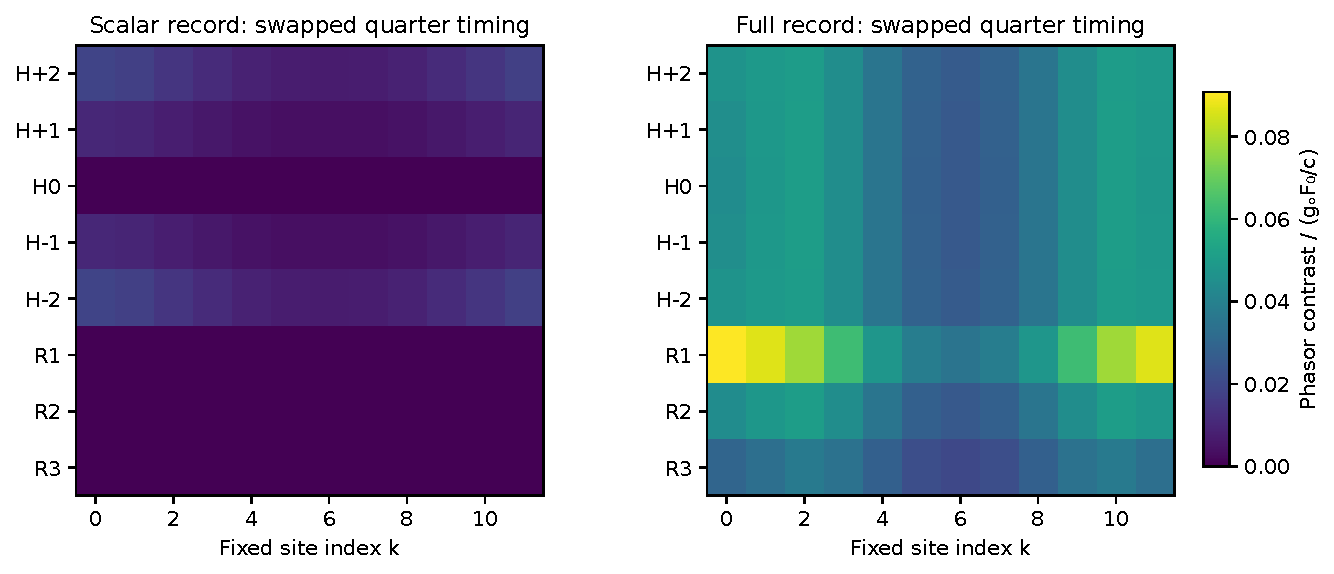
\includegraphics[width=\textwidth]{figures/exterior.pdf}
\caption{Scalar versus full exterior contrast, redrawn from retained SRG-06--08 data. Equatorial scalar rows have exact zero contrast for exchanged direction/timing; directional records remain distinct. Horizontal indices are fixed sites, not time. Common calibration is retained, and no entry is normalized separately.}\label{fig:exterior}
\end{figure}

\subsection{Phasors, snapshots, calibration and squared records}\label{sec:information}
Complex rank two identifies two complex amplitudes with a known clock and gain, equivalently their full-period records at known nonzero frequency. An unknown common nonzero complex factor leaves the ratio $a_-/a_+$ identifiable after a rank-two inverse, but removes absolute scale and common phase. Its modulus gives $\Jflux/(cE)$ for the mean-free family. If separate unknown factors multiply each scalar site, they can absorb the height phase contrast site by site. A full single site still has a projective inverse when one factor is common to all its channels; independent channel factors or an unknown frame remove that guarantee.

One real snapshot instead maps four real amplitude coordinates through $[\Re Q,-\Im Q]$, up to a common time phase. One site has at most three real channels and cannot invert four real unknowns. The retained finite stack results are:
\begin{table}[htbp]\centering
\begin{tabular}{lcc}\toprule
Stack & Scalar real rank, $\nu=0/1$ & Full real rank, $\nu=0/1$\\\midrule
Each off-height H ring &2 / 4&4 / 4\\
Each equatorial ring &1 / 2&3 / 4\\
H or unique union &2 / 4&4 / 4\\
R &1 / 2&3 / 4\\\bottomrule
\end{tabular}
\caption{Inherited snapshot classifications for the all-time first-harmonic family. Finite-delay full-rank statements here are finite numerical findings; the smallest reported nonzero singular value exceeds .005.}\label{tab:snapshots}
\end{table}
At zero delay, the scalar snapshot contains only the two real spatial coefficients of $p$, and an equatorial vector record misses one real coefficient of $r$, explaining the exact upper bounds. Retarded samples can contain additional quadratures in this assumed family. This is not instantaneous reconstruction of arbitrary histories.

\begin{proposition}[Squared-record blindness]\label{prop:power}
For T+ and T-, scalar phasor magnitudes and full phasor squared norms agree at every off-circle site and every delay. For the standing controls,
\begin{equation}\label{eq:scalarpower}
 |\widehat U_{S0}|^2=g_o^2A_0^2|H|^2\cos^2\phi,\qquad
 |\widehat U_{S45}|^2=g_o^2A_0^2|H|^2\cos^2(\phi-\pi/4).
\end{equation}
Individual directional-component period mean squares can differ at finite delay.
\end{proposition}
\begin{proof}
For either traveller, $|z_+|=|z_-|=A_0/\sqrt2$. Orthogonality in \eqref{eq:reduction} makes scalar and total squared norms identical. Substituting the two standing amplitudes gives the cosine factors in \eqref{eq:scalarpower}. For a real local component, set $q_j=(B\tr e_q)_j$ and $t_j=(B\tr e_\perp)_j$. The two vector column entries differ by the sign of the $C_mt_j$ term. Expanding their squared moduli and multiplying by the traveller amplitude square and the period factor $1/2$ gives
\begin{equation}\label{eq:componentpower}
 \langle Y_{j,T+}^2\rangle-\langle Y_{j,T-}^2\rangle
 =g_o^2A_0^2\Re(\ii S_m\overline{C_m})q_jt_j.
\end{equation}
At zero delay the moments are real, so this vanishes. Summing components also gives zero because $e_q\cdot e_\perp=0$.
\end{proof}
At H+1:00 and $\nu=1$, the inherited component differences $(U,V_1,V_2,V_3)$ are $(0,-8.21792406\times10^{-5},+8.21792406\times10^{-5},0)$ for $g_o=A_0=1$. At equatorial sites the products $q_jt_j$ vanish in the retained frames. These are calibrated readout statistics, not emitted or absorbed power.

\subsection{Causal composition and possible arrival}\label{sec:causality}
From zero preparation at $t_0$, substitution of \eqref{eq:characteristics} into C6 gives
\begin{equation}\label{eq:composition}
 \begin{split}
 Y_X(t)=\frac{g_o}{8\pi}\sum_{j=\pm}\sum_{\sigma=\pm1}
 \int_\Gamma\frac{1}{d_X(s)}\binom{1}{\sigma B\tr\hat t(s)}\hspace{-1mm}
 \int_{t_0}^{t-d_X(s)/c_e}
 b_j\big(s-\sigma c[t-d_X(s)/c_e-u]\big)f_j(u)\dd u\dd s .
 \end{split}
\end{equation}
An inner integral with upper endpoint below $t_0$ is zero. Compact forcing can also truncate its upper endpoint at switch-off. The $1/2$ splitting follows from the two characteristic conversions and is not an adjustable gain.

\begin{proposition}[Support-arrival infimum]\label{prop:arrival}
For source support $S_j$ beginning at $t_0$, the first possible support arrival obeys
\begin{equation}\label{eq:arrival}
 t_0+\inf_{u\in S_j,\ s\in\Gamma,\ \sigma=\pm1}
 \left\{\frac{D_\sigma(u,s)}c+\frac{d_X(s)}{c_e}\right\}.
\end{equation}
If $c\le c_e$, this infimum equals $t_0+\inf_{u\in S_j}d_X(u)/c_e$.
\end{proposition}
\begin{proof}
The inner source integrand in \eqref{eq:composition} can contribute only after a characteristic has travelled from its support to $s$, followed by the exterior delay from $s$ to $X$. Taking the least directed arc and then the infimum gives \eqref{eq:arrival}; further windings add $L/c$. For $c\le c_e$, arc length exceeds chord length, so
\[
 \frac{D_\sigma(u,s)}c+\frac{d_X(s)}{c_e}
 \ge\frac{\norm{\Gamma(s)-\Gamma(u)}+d_X(s)}{c_e}
 \ge\frac{d_X(u)}{c_e}.
\]
Choosing $s=u$ gives equality of the infima. If $c>c_e$, the first inequality need not hold, and no such reduction is asserted.
\end{proof}
Tent edges, smooth source onset, zero integration length and scalar/vector cancellations can prevent nonzero measurement at the threshold. A parity-blind channel may remain zero forever. The calculation is about finite support, not a contact-centre shortcut. C6 changes no term in $\dot E$; neither a squared record nor its sum is a debit from the carrier.

\section{A finite paired pulse generates a standing residual}\label{sec:pulse}
The preceding free waves were independently prepared. We next derive what the retained source interface generates from rest under the SRG-07 calibration.~\cite{SRG07} Fix $\epsilon=L/32$, $T=L/c$, $\omega=c/R=2\pi/T$, and
\begin{equation}\label{eq:pulse}
 h(t)=\begin{cases}\sin^2(\pi t/T),&0\le t\le T,\\0,&\text{otherwise},\end{cases}
 \qquad f_\pm(t)=(F_s\pm F_a)h(t),\qquad p=r=0\quad(t\le0).
\end{equation}
Here $F_s,F_a$ are real constants. The zero extension is $C^1$, since both $h$ and $h'$ vanish at the endpoints. Its exactly one-circuit duration is a temporal calibration, not a native drive period. Define $C_g=\sqrt{3/7}$, $S_g=2/\sqrt7$ and $B_n=\sinc^2(n\pi/32)$, with $b=B_1=0.996791364044961\ldots$.

The controls S, A, M+, M- and ZERO use
\begin{equation}\label{eq:pulsecontrols}
 (F_s,F_a)/F_0=(1,0),(0,1),(1,1)/\sqrt2,(1,-1)/\sqrt2,(0,0)
\end{equation}
with one common $F_0>0$. M+ is upper-only, M- lower-only. They are names for pulse combinations, not additional native macro families. Expanding $f_+^2+f_-^2$ and integrating $\sin^4$ gives
\begin{equation}\label{eq:drivenorm}
 \int_0^T(f_+^2+f_-^2)\dd t=\frac{3T}{4}(F_s^2+F_a^2).
\end{equation}
All four nonzero controls have equal squared drive norm, which does not imply equal signed work.

\subsection{All modes during forcing; exact cancellation at switch-off}
Let $G=(F_s+F_a)b_++(F_s-F_a)b_-$. Its Fourier coefficients are
\begin{equation}\label{eq:G}
 G_n=\frac{2(-1)^n}{L}B_n[F_s\cos(n\theta)+\ii F_a\sin(n\theta)].
\end{equation}
For $0\le v\le T$, introduce the entire limiting primitive
\begin{equation}\label{eq:J}
 E_m(v)=\begin{cases}(e^{\ii m\omega v}-1)/(\ii m\omega),&m\ne0,\\v,&m=0,\end{cases}
 \qquad J_n(v)=\tfrac12E_n(v)-\tfrac14E_{n+1}(v)-\tfrac14E_{n-1}(v).
\end{equation}
For $t\ge0$ set $v=\min(t,T)$ and $Z_n=e^{-\ii n\omega t}J_n(v)$. Direct use of the two characteristics gives
\begin{equation}\label{eq:transient}
 p_n(t)=G_n\Re Z_n,\qquad r_n(t)=\ii G_n\Im Z_n,
 \qquad p_0(t)=\frac{F_s}{L}\left(v-\frac{\sin\omega v}{\omega}\right),\quad r_0=0.
\end{equation}
The spatial form, with periodic arguments, is
\begin{equation}\label{eq:directpulse}
 \binom p r(s,t)=\frac12\sum_{\sigma=\pm1}\binom1\sigma
 \int_0^{\min(t,T)}G(s-\sigma c(t-u))h(u)\dd u.
\end{equation}
These formulas retain the full spatial spectrum. The finite tent is not a hard cutoff, and generally $J_n(v)\ne0$ for higher modes before switch-off.

\begin{theorem}[One-circuit pulse selection]\label{thm:pulsemoments}
For every integer $n$ and $\sigma=\pm1$,
\begin{equation}\label{eq:pulsemoments}
 \int_0^T h(u)e^{\sigma\ii n\omega u}\dd u
 =\frac T2\delta_{n0}-\frac T4(\delta_{n1}+\delta_{n,-1}).
\end{equation}
Consequently at $t=T$,
\begin{equation}\label{eq:switchoff}
 p_0=F_s/c,\quad r_n=0\ (n\in\mathbb Z),\quad
 p_1=\frac b{2c}(F_sC_g+\ii F_aS_g),\quad p_{-1}=\overline{p_1},\quad p_n=0\ (|n|\ge2).
\end{equation}
\end{theorem}
\begin{proof}
Write $h(u)=1/2-e^{\ii\omega u}/4-e^{-\ii\omega u}/4$ on its support. Every nonconstant integer exponential integrates to zero on $[0,T]$; the constant integrates to $T$. Applying this to each of the three terms gives \eqref{eq:pulsemoments} for every integer, including $0,\pm1$. There is no singular denominator: its value is precisely the $E_0$ branch of \eqref{eq:J}. At $T$, all free phase factors $e^{\pm\ii n\omega T}$ equal one, and the two signed moments agree. Thus their half-difference, the $r_n$ coefficient, is zero. Their half-sum gives $p_n=G_nJ_n(T)$. Substituting \eqref{eq:G} at $n=0,1$ gives \eqref{eq:switchoff} and real conjugacy gives $n=-1$.
\end{proof}

\begin{corollary}[Uniquely generated continuation]\label{cor:standing}
For $\tau=t-T\ge0$, the resulting free continuation is
\begin{equation}\label{eq:residual}
 \begin{aligned}
 p&=\frac{F_s}{c}+\frac bc(F_sC_g\cos\chi-F_aS_g\sin\chi)\cos\omega\tau,\\
 r&=\frac bc(F_sC_g\sin\chi+F_aS_g\cos\chi)\sin\omega\tau.
 \end{aligned}
\end{equation}
At the shared $T$ reference its first-harmonic amplitudes are
\begin{equation}\label{eq:pulseamplitudes}
 a_+=\frac b{2c}(F_sC_g-\ii F_aS_g),\qquad
 a_-=\frac b{2c}(F_sC_g+\ii F_aS_g).
\end{equation}
\end{corollary}
\begin{proof}
The mean is constant after forcing. Evolving each surviving Fourier coefficient with unforced C1 gives $p_1(T+\tau)=p_1(T)\cos\omega\tau$ and $r_1(T+\tau)=-\ii p_1(T)\sin\omega\tau$. Combining conjugate spatial modes gives \eqref{eq:residual}; comparison with \eqref{eq:freefamily} gives \eqref{eq:pulseamplitudes}. It matches the complete switch-off state and solves C1, so uniqueness identifies it as the continuation.
\end{proof}

Here $a_-=p_1(T)$, not $a_+$. For real $F_s,F_a$, the amplitudes are conjugates and their magnitudes agree. S produces a mean plus cosine standing pattern; A produces a mean-free sine standing pattern. M$\pm$ yield standing $p$ harmonics proportional to $\cos(\chi\pm\theta)$. The shift records contact geometry, not opposite circulation. Higher-mode cancellation is a property of the completed pulse and its exact duration; it is neither damping nor a universal selection law.

\begin{theorem}[Common-envelope obstruction at every time]\label{thm:commonzero}
For zero preparation and any real separable forcing $G(s)h(t)$ with the finite-profile regularity above, $\Jflux(t)=0$ at every time, including during forcing. This includes all controls in \eqref{eq:pulsecontrols}.
\end{theorem}
\begin{proof}
The modal Duhamel solution has $p_n=G_n A_n$ and $r_n=-\ii G_n B_n^{\rm time}$, where $A_n=\int_0^t h(u)\cos[ck_n(t-u)]\dd u$ and $B_n^{\rm time}=\int_0^t h(u)\sin[ck_n(t-u)]\dd u$ are real. Hence $\Re(p_n\overline{r_n})=0$ for every mode. The mean $r_0$ is zero. Parseval, justified by $L^2$ convergence and Cauchy--Schwarz for the coefficient product, gives $c\int pr\dd s=0$. This proves an all-time statement, stronger than equality of the two residual magnitudes. Local flux need not vanish.
\end{proof}

\subsection{Signed work, storage and port interference}
\begin{proposition}[Pulse work and storage]\label{prop:pulsework}
For \eqref{eq:pulse}, the final storage and integrated signed source work are
\begin{equation}\label{eq:pulsestorage}
 E_f=W_{\rm src}=\frac L{c^2}\left[\frac12F_s^2+
 \frac{b^2}{4}(C_g^2F_s^2+S_g^2F_a^2)\right].
\end{equation}
The antisymmetric control A has negative instantaneous source work on an interval immediately before $T$, although its total work is positive.
\end{proposition}
\begin{proof}
Integrating the square of \eqref{eq:residual} uses $\int\sin\chi=\int\cos\chi=\int\sin\chi\cos\chi=0$ and $\int\sin^2\chi=\int\cos^2\chi=L/2$. The mean/harmonic and symmetric/antisymmetric cross terms vanish by these identities, giving the displayed $E_f$.

Independently integrate the actual source work. Put $I_n=J_n(T)$ and define
\[
 A_n(t)=\int_0^t h(u)\cos[n\omega(t-u)]\dd u.
\]
The source power is $Lh(t)\sum_n|G_n|^2A_n(t)$. Symmetry of the cosine kernel gives
\[
 \int_0^T h(t)A_n(t)\dd t
 =\frac12\int_0^T\int_0^T h(t)h(u)\cos[n\omega(t-u)]\dd u\dd t
 =\frac12|I_n|^2.
\]
Thus $W_{\rm src}=(L/2)\sum_n|G_n|^2|I_n|^2$. The finite-profile coefficient decay and bounded temporal integrals justify interchanging sum and integrals. Inserting \eqref{eq:pulsemoments} produces exactly \eqref{eq:pulsestorage}, without defining work by endpoint storage.

Before multiplication by the endpoint envelope, the limiting source trace is
\begin{equation}\label{eq:negativework}
 \int Gp(T)\dd s=\frac2c\left[F_s^2-b^2(C_g^2F_s^2+S_g^2F_a^2)\right].
\end{equation}
This follows by pairing the mean and first harmonics of $G$ and $p(T)$. For A it is $-2b^2S_g^2F_0^2/c<0$. The trace is continuous in time, and $h(t)>0$ just before $T$. Hence $h(t)\int Gp(t)\dd s<0$ on a final open interval. The endpoint itself has zero power because $h(T)=0$.
\end{proof}

For S and the positive single-port controls, $G\ge0$, and \eqref{eq:directpulse} implies $p\ge0$. Their instantaneous work is nonnegative. These different signs arise from the prescribed sources, with no negative storage. The comparison in Table~\ref{tab:pulsestorage} uses a single unit $F_0^2L/c^2$.
\begin{table}[htbp]\centering
\begin{tabular}{lrrr}\toprule
Control & Mean storage & Harmonic storage & Total storage / signed work\\\midrule
S & .5000000000 & .1064563954 & .6064563954\\
A & 0 & .1419418605 & .1419418605\\
M+ & .2500000000 & .1241991279 & .3741991279\\
M- & .2500000000 & .1241991279 & .3741991279\\
ZERO & 0 & 0 & 0\\\bottomrule
\end{tabular}
\caption{Same squared drive norm for nonzero controls; unequal delivered work. The A/S harmonic-storage ratio is exactly $4/3$, but S has larger total storage because its mean remains.}\label{tab:pulsestorage}
\end{table}

Let $\alpha_S=1/2+3b^2/28$ and $\alpha_A=b^2/7$. In terms of actual port amplitudes $F_\pm=F_s\pm F_a$, the account becomes
\begin{equation}\label{eq:portcross}
 E_f=\frac L{4c^2}\left[(\alpha_S+\alpha_A)(F_+^2+F_-^2)
 +2(\alpha_S-\alpha_A)F_+F_-\right].
\end{equation}
Thus diagonalization in reflection sectors does not make physical port work independent. The mixed term is nonzero and cannot be replaced by absolute values.

\begin{figure}[htbp]\centering
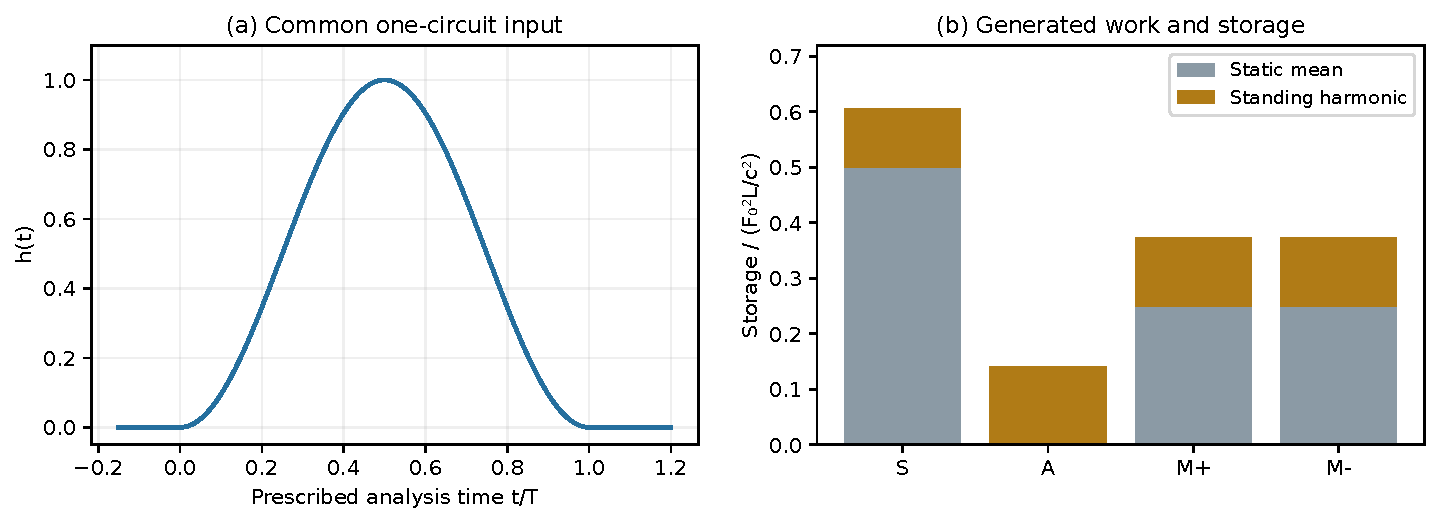
\includegraphics[width=\textwidth]{figures/pulse.pdf}
\caption{Common-pulse calibration and its generated storage, from retained SRG-07 data. The waveform is a prescribed input, not a simulated native trajectory. Bars retain the static mean and share the unit $F_0^2L/c^2$. All four nonzero cases have zero integrated directional bias at all times.}\label{fig:pulse}
\end{figure}

\subsection{Complete late records and the two-real-coefficient inverse}
Across the full fixed array,
\begin{equation}\label{eq:latewindow}
 D_{\max}=4+K+R=5.29316210017650\ldots,\qquad
 I_{\rm late}=[T+D_{\max}/c_e,T+D_{\max}/c_e+T].
\end{equation}
The maximum is attained at R3:06. Since $d_X(s)\le D_{\max}$, every retarded argument in this common window is at least $T$. At zero exterior delay the additional offset is zero. The phase reference remains $t-T$ at every site; it is not aligned independently to local delay.

Use the accepted unit-$g_o$ matrices $Q_X(\nu)$ and the accepted zero-delay moments to define
\begin{equation}\label{eq:sourceN}
 N=\frac b2\begin{pmatrix}C_g&-\ii S_g\\C_g&\ii S_g\end{pmatrix},\quad
 D_X=S_m(X,0)+C_m(X,0)=\frac1{4\pi}\int_\Gamma d_X^{-1}\dd s>0.
\end{equation}
For $\mathbf f=(F_s,F_a)\tr/F_0$, the complete late record is
\begin{equation}\label{eq:laterecord}
 \frac{Y_X(t)}{g_oF_0/c}
 =\begin{pmatrix}D_X&0\\0&0\\0&0\\0&0\end{pmatrix}\mathbf f
 +\Re\{Q_X(\nu)N\mathbf f\,e^{\ii\omega(t-T)}\}.
\end{equation}
There is no static vector term because $\bar r=0$. Earlier records require \eqref{eq:composition} with the actual pulse, including its transient higher modes; the late expression is not a prehistory substitute.

\begin{theorem}[Causal null and calibrated pulse identification]\label{thm:pulseinverse}
Under the common-pulse controls, equatorial scalar reception satisfies $U_A=0$ and $U_{M+}=U_{M-}=U_S/\sqrt2$ throughout the causal history, for every $c_e$. At $\nu=0,1$, a full harmonic record at any retained site identifies both real coefficients $F_s,F_a$. A single off-height scalar harmonic has only real rank one, while its calibrated DC-plus-harmonic record has real rank two. The fixed off-height mirror pair or each off-height H ring has harmonic scalar rank two. Coplanar scalar stacks have rank one even with DC.
\end{theorem}
\begin{proof}
Proposition~\ref{prop:parity} makes $p_A$ odd under $s\mapsto L-s$. At an equatorial site the distance and delay are even under that reflection, so opposite source points are read at the same time and cancel. Linearity gives the M$\pm$ identity for the entire history.

Substitute \eqref{eq:pulseamplitudes} into \eqref{eq:reduction}. In the common scale the scalar harmonic is
\begin{equation}\label{eq:pulsescalar}
 \widehat U/(g_oF_0/c)=bH(C_g f_s^{\rm norm}\cos\phi-S_g f_a^{\rm norm}\sin\phi),
\end{equation}
where $f_s^{\rm norm}=F_s/F_0$, $f_a^{\rm norm}=F_a/F_0$. This is one real combination times a known complex scalar, so it has real rank one. At off-height sites $\sin\phi\ne0$; DC determines $F_s$ since $D_X>0$, after which \eqref{eq:pulsescalar} determines $F_a$. The two mirror harmonic rows are proportional to $(C_g\cos\phi,\mp S_g\sin\phi)$, both factors nonzero at the declared pair. The same nonparallel-angle argument as in Theorem~\ref{thm:height} treats each off-height ring. At equator the $F_a$ column vanishes, including DC. Finally $\det N=\ii b^2C_gS_g/2\ne0$ and $Q_X$ has complex rank two. Hence $Q_XN$ is injective even over $\C^2$, in particular on the two real coefficients.
\end{proof}

At equator the antisymmetric vector harmonic is explicitly
$\widehat V_A/(g_oF_0/c)=-\ii bS_gC_m\ez\ne0$. It occupies local component 2 in the inherited frame. Thus a source-generated field with no net directional bias can still have a nonzero directional record and an exactly zero scalar record. Distinguishing an input does not itself detect circulation.

The new inverse has two real unknowns; it is not the earlier four-real-dimensional free-wave problem. An unknown common gain removes absolute source/work calibration. A common unknown harmonic phase still leaves a ratio after a full-channel or independent scalar-stack inverse, but a single off-height scalar DC-plus-harmonic detector needs its stated phase calibration: the sign of its one harmonic combination can otherwise be ambiguous. Independent site/channel gains and clocks require additional assumptions; none are estimated here.

\subsection{Retained source-response errors and scope}\label{sec:pulseerrors}
The old reception matrices are reused at $\nu=0,1$. Their composition is a new source-to-record interpretation, not a repeated quadrature. The source matrix has $\norm N_2=0.532807395764471\ldots$. Thus
\begin{equation}\label{eq:compositionerror}
 \norm{\delta(Q_XN)}_F\le\norm{\delta Q_X}_F\norm N_2
 +\text{source-map and output rounding allowances}.
\end{equation}
DC error is the sum of the two zero-delay moment errors and serialization allowance. The retained complete per-site allowance is at most $2.700\times10^{-14}$; stack allowances combine in quadrature, with a separate $10^{-11}$ allowance for numerical matrix summaries. These remain non-interval qualifications. For example, the complete scalar smallest singular values of H are $.01027058/.04942127$ at $\nu=0/1$, whereas R has an exact zero; full harmonic values are $.22860363/.22678517$ for H and $.20912274/.20388032$ for R. The figures and data retain the common normalization.

The original six characteristic-point checks and their tail estimates remain inherited evidence, not an all-mode proof or a newly executed suite. The all-integer cancellation is proved in Theorem~\ref{thm:pulsemoments}; the all-time null in Theorem~\ref{thm:commonzero}; the causal scalar blindness in Theorem~\ref{thm:pulseinverse}. These do not infer a native generating trajectory, recover $W_a$ or $J$, or equate the observation statistics with receiver energy.

\section{Temporal cross-phase and generated directional imbalance}\label{sec:timing}
The common-envelope obstruction suggests a general question before selecting any lag: which temporal relationship between two source histories creates an imbalance? The answer combines their finite-time cross-phase with the actual contact angle.~\cite{SRG08} Throughout this section preparation is zero and the mean is retained.

\subsection{General finite-history theorem}
Let real $f_\pm$ have support in $[0,\tf]$ and belong to $L^2$ there; continuous or piecewise continuous histories suffice. Put $\omega_n=nc/R$ and
\begin{equation}\label{eq:finiteF}
 \F_j(\omega)=\int_0^{\tf}f_j(u)e^{+\ii\omega u}\dd u,\qquad
 \F_j^t(\omega)=\int_0^{\min(t,\tf)}f_j(u)e^{+\ii\omega u}\dd u,
 \qquad\beta_n=B_n/L.
\end{equation}
The value at zero is the actual integral. Use one common reference $\tref\ge\tf$ for post-source amplitudes, with the convention
\begin{equation}\label{eq:generalexpansion}
 \begin{aligned}
 p&=\bar p+\sum_{n\ge1}\Re\{(a_{+,n}e^{-\ii n\chi}+a_{-,n}e^{\ii n\chi})e^{\ii\omega_n(t-\tref)}\},\\
 r&=\bar r+\sum_{n\ge1}\Re\{(a_{+,n}e^{-\ii n\chi}-a_{-,n}e^{\ii n\chi})e^{\ii\omega_n(t-\tref)}\}.
 \end{aligned}
\end{equation}

\begin{theorem}[Temporal cross-phase criterion]\label{thm:temporal}
Under these assumptions,
\begin{equation}\label{eq:generalamp}
 a_{\sigma,n}=\beta_ne^{\ii\omega_n\tref}
 \sum_{j=\pm}e^{\sigma\ii ns_j/R}\overline{\F_j(\omega_n)},\qquad
 \bar p=\frac{\F_+(0)+\F_-(0)}L,\quad\bar r=0.
\end{equation}
For each positive $n$, the squared-amplitude difference is
\begin{equation}\label{eq:criterion}
 \boxed{D_n=|a_{+,n}|^2-|a_{-,n}|^2
 =-4\beta_n^2\sin(2n\theta)\Im(\F_+\overline{\F_-})
 =8\beta_n^2\sin(2n\theta)\Im(\F_s\overline{\F_a}).}
\end{equation}
The same identities with truncated transforms hold at each finite time. Furthermore,
\begin{equation}\label{eq:generalaccount}
 E=\frac L2\bar p^2+\sum_{n\ge1}\frac L2(|a_{+,n}|^2+|a_{-,n}|^2),\qquad
 \Jflux=\frac{cL}2\sum_{n\ge1}D_n.
\end{equation}
The series converge; a nonzero term $D_n$ need not imply a nonzero signed sum.
\end{theorem}
\begin{proof}
Multiply \eqref{eq:characteristics} by $\sqrt2$. The unnormalized variable $p+\sigma r$ equals the sum over ports of $\int b_j(s-\sigma c(t-u))f_j(u)\dd u$. Its spatial Fourier coefficient is
$\beta_n\sum_j e^{-\ii ns_j/R}e^{-\sigma\ii\omega_nt}\F_j(\sigma\omega_n)$.
For real inputs $\F_j(-\omega)=\overline{\F_j(\omega)}$. In $p$, recombination contributes $1/2$, whereas expressing a real harmonic as a real part contributes a factor 2. They cancel. Selecting the spatial mode with positive temporal frequency gives exactly \eqref{eq:generalamp}; this verifies the absence of an extra factor of two. The zero mode follows directly by averaging C1.

To check the sign, set $Z=\F_+\overline{\F_-}$ and $d_n=n(s_+-s_-)/R=-2n\theta$. Expanding the cross terms in the squared moduli of \eqref{eq:generalamp} gives
$2\beta_n^2[\Re(e^{\ii d_n}\overline Z)-\Re(e^{-\ii d_n}\overline Z)]
=4\beta_n^2\sin d_n\Im Z$.
This is the first equality in \eqref{eq:criterion}. Since $\F_\pm=\F_s\pm\F_a$, one has $\Im(\F_+\overline{\F_-})=-2\Im(\F_s\overline{\F_a})$, giving the second.

For every truncated time, $|\F_j^t|\le\norm{f_j}_{L^1}\le\sqrt{\tf}\norm{f_j}_{L^2}$. The profile gives $\beta_n=O(n^{-2})$, uniformly bounding amplitudes by a summable sequence. Thus the field series converges absolutely and its storage/flux terms have summable $O(n^{-4})$ bounds. Orthogonality between distinct spatial modes and cancellation of opposite-direction cross terms between $p^2$ and $r^2$ give \eqref{eq:generalaccount}, as in Proposition~\ref{prop:freeenergy}. The same calculation at a finite time uses truncated transforms. The mild solution and integrated balance accommodate jumps in a sample-and-hold input; time differentiability is then asserted only almost everywhere. Nothing permits replacing the signed mode sum by the magnitude of one term.
\end{proof}

\begin{corollary}[Obstructions and covariance]\label{cor:temporalzeros}
One-port inputs and proportional real histories have $D_n=0$ at every truncated time. A common time translation preserves residual imbalance. Exchanging the physical port histories reverses every $D_n$ while preserving storage and mean. Arclength reversal instead relabels orientation and changes the sign assigned to the same geometric flux.
\end{corollary}
\begin{proof}
For one port the cross product is zero; for $f_-=kf_+$ with real $k$, it is $k|\F_+^t|^2$, which is real at every time. Translating both histories multiplies their transforms by the same $e^{\ii\omega\tau}$ and leaves the product unchanged. Exchanging them conjugates the product, reversing its imaginary part. In the actual reflected geometry \eqref{eq:generalamp} exchanges the two directional amplitudes and leaves the means unchanged. Coordinate reversal instead sends $r\mapsto-r$ and interchanges the characteristic labels, as established for C6. It does not exchange the physical drive schedules.
\end{proof}

Nonproportionality alone is insufficient: the cross product may be real at carrier eigenfrequencies or its modal contributions may cancel in the signed sum. Profile zeros at $n=32m\ne0$ and arbitrarily small coupling factors remain. No uniform inverse bound follows from the irrational-angle nonvanishing theorem.

\subsection{Fixed shifted controls at a common phase origin}
Only now select the already accepted timing comparisons. All use the same $h$ in \eqref{eq:pulse}, zero preparation, and $\tref=3T/2$:
\begin{table}[htbp]\centering\small
\begin{tabular}{lccc}\toprule
Control & $f_+/F_0$ & $f_-/F_0$ & Last switch-off\\\midrule
CO &$h(t)$&$h(t)$&$T$\\
Lower late Q &$h(t)$&$h(t-T/4)$&$5T/4$\\
Upper late Q &$h(t-T/4)$&$h(t)$&$5T/4$\\
Lower late H &$h(t)$&$h(t-T/2)$&$3T/2$\\
One upper &$\sqrt2h(t)$&$0$&$T$\\
ZERO &$0$&$0$&$0$\\\bottomrule
\end{tabular}
\caption{The five nonzero controls share integrated squared drive norm $3F_0^2T/4$. Q and H denote the fixed quarter- and half-period delays, not adjusted outcomes.}\label{tab:schedules}
\end{table}
No source is restarted when the other begins. For a delay $d$, substitution $u=v+d$ gives the completed moment $e^{\ii\omega_nd}I_n$ with $I_n$ from \eqref{eq:pulsemoments}. During forcing the moment is $e^{\ii\omega_nd}J_n(v)$, where $v$ is clamped to $[0,T]$. Thus a completed shift does not repopulate higher residual modes, while the transient still can contain them.

For any first-harmonic residual, changing reference from $t_0$ to $t_1$ multiplies its amplitude by $e^{\ii\omega(t_1-t_0)}$, because the product with $e^{\ii\omega(t-t_1)}$ must stay unchanged. In particular the SRG-07 $T$-reference amplitudes acquire a minus sign at $3T/2$. No individual control or observer is rephased to simplify the result.

\begin{proposition}[Generated delayed-pulse account]\label{prop:lag}
For the lower-late input $F_0h(t),F_0h(t-\Delta)$ with $0\le\Delta\le T/2$, set $\alpha=\omega\Delta$. At reference $3T/2$,
\begin{equation}\label{eq:lagamp}
 \bar p=F_0/c,\quad\bar r=0,\quad
 a_+=-\frac{bF_0}{4c}(e^{-\ii\theta}+e^{\ii\theta-\ii\alpha}),\quad
 a_-=-\frac{bF_0}{4c}(e^{\ii\theta}+e^{-\ii\theta-\ii\alpha}).
\end{equation}
All residual $|n|\ge2$ vanish. In units $F_0^2L/c^2$,
\begin{equation}\label{eq:lagenergy}
 \begin{aligned}
 E_\pm&=\frac{b^2}{16}[1+\cos(2\theta\mp\alpha)],\quad E_{\rm mean}=\tfrac12,\\
 E_{\rm osc}&=\frac{b^2}{8}(1-\cos\alpha/7),\quad
 \Delta E=E_+-E_-=\frac{b^2}{8}\sin(2\theta)\sin\alpha.
 \end{aligned}
\end{equation}
When their denominators are nonzero, the two distinct imbalance ratios are
\begin{equation}\label{eq:etas}
 \eta_{\rm osc}=\frac{\sin(2\theta)\sin\alpha}{1-\cos\alpha/7},\qquad
 \eta_{\rm total}=\frac{b^2\sin(2\theta)\sin\alpha}{4+b^2(1-\cos\alpha/7)}.
\end{equation}
\end{proposition}
\begin{proof}
The zero-frequency moment of each source is $F_0T/2$, so \eqref{eq:generalamp} gives the mean. Only $n=1$ remains for positive indices. Insert $I_1=-T/4$, the lower-port shift $e^{\ii\alpha}$, $s_\pm/R=\pi\mp\theta$, and $e^{\ii\omega(3T/2)}=-1$ into \eqref{eq:generalamp}. This gives \eqref{eq:lagamp}, including its leading minus. Squaring the sums uses $|e^{\ii x}+e^{\ii y}|^2=2+2\cos(x-y)$. Apply \eqref{eq:generalaccount} and $\cos(2\theta)=-1/7$ to obtain \eqref{eq:lagenergy}. Dividing $\Delta E$ by the harmonic or total storage gives \eqref{eq:etas}; the mean must not be dropped from the second denominator.
\end{proof}

For the quarter pair,
\begin{equation}\label{eq:quarter}
 (a_+,a_-)_{\rm LQ}=-\frac{bF_0}{4c}(1-\ii)(C_g+S_g,C_g-S_g),
 \qquad \frac{a_-}{a_+}=4\sqrt3-7=-0.07179677\ldots .
\end{equation}
The ratio is nonzero: the wave is strongly biased, not a pure traveller. Upper late exchanges these amplitudes. CO gives $a_+=a_-=-bF_0C_g/(2c)$; half-late gives $(a_+,a_-)=(\ii bF_0S_g/(2c),-\ii bF_0S_g/(2c))$. One upper gives $a_\pm=-bF_0e^{\mp\ii\theta}/(2\sqrt2c)$ and mean $F_0/(\sqrt2c)$.

\begin{table}[htbp]\centering\small
\begin{tabular}{lrrrrrr}\toprule
Control & $E_{\rm mean}$ & $E_+$ & $E_-$ & $E_{\rm total}$ & $\eta_{\rm osc}$ & $\eta_{\rm total}$\\\midrule
CO &.500000&.05322820&.05322820&.60645640&0&0\\
Lower late Q &.500000&.12356219&.00063694&.62419913&.98974332&.19693276\\
Upper late Q &.500000&.00063694&.12356219&.62419913&$-.98974332$&$-.19693276$\\
Lower late H &.500000&.07097093&.07097093&.64194186&0&0\\
One upper &.250000&.06209956&.06209956&.37419913&0&0\\
ZERO &0&0&0&0&undefined&undefined\\\bottomrule
\end{tabular}
\caption{Inherited fixed timing controls in common storage units $F_0^2L/c^2$. Total storage equals independently integrated signed work. Zero-state normalized imbalances are undefined.}\label{tab:timing}
\end{table}

The lower-late harmonic imbalance is $4\sqrt3/7=98.9743\%$, whereas its total-storage imbalance is $19.6933\%$. Its positive-direction fraction of harmonic storage is $(1+\eta_{\rm osc})/2=99.4872\%$. These three figures describe different ratios; none is decoding accuracy, speed or a capacity measurement.

\begin{proposition}[Balanced residual does not imply balanced history]\label{prop:halftime}
The half-period delayed control has zero residual integrated flux, but at $t=T$,
\begin{equation}\label{eq:halftransient}
 \frac{\Jflux(T)}{F_0^2L/c}=\frac{b^2\sin(2\theta)}{4\pi}>0.
\end{equation}
\end{proposition}
\begin{proof}
At $t=T$ the upper source is complete and the lower source is half complete. Evaluating \eqref{eq:J} gives
$\F_+^T(\omega)=-F_0T/4$ and $\F_-^T(\omega)=F_0[T/8-\ii T/(2\pi)]$.
Their cross product has imaginary part $-F_0^2T^2/(8\pi)$. Insert it into \eqref{eq:criterion} at $n=1$, multiply by $cL/2$ and use $T=L/c$. At every $n\ge2$ the completed upper moment is zero, so all other cross terms vanish at this instant. The mean has no flux. This proves that the displayed first-harmonic value is the complete signed sum at $T$. At $3T/2$ the completed relative phase is $\pi$, so \eqref{eq:lagenergy} gives zero residual bias.
\end{proof}

The half-late and CO controls therefore agree only in final directional balance; their phases, storage and causal histories differ. Nonproportional histories need not give nonzero terminal bias, and a zero terminal bias need not persist at earlier times.

\subsection{Work derived from the time-ordered source integral}\label{sec:timingwork}
For arbitrary finite histories put $S_n(t)=\beta_n\sum_j e^{-\ii ns_j/R}f_j(t)$. Modal Duhamel gives $p_n(t)=\int_0^tS_n(u)\cos[\omega_n(t-u)]\dd u$. The mean contributes $W_0=L|\int S_0|^2/2$. For $n>0$, the signed work of the conjugate spatial pair is
\begin{equation}\label{eq:generalwork}
 \begin{aligned}
 W_n&=2L\Re\int_0^{\tf}\overline{S_n(t)}\int_0^tS_n(u)\cos[\omega_n(t-u)]\dd u\dd t\\
 &=\frac L2\left(\left|\int_0^{\tf}S_n(u)e^{\ii\omega_nu}\dd u\right|^2
 +\left|\int_0^{\tf}S_n(u)e^{-\ii\omega_nu}\dd u\right|^2\right).
 \end{aligned}
\end{equation}
To prove the second equality, reflect the ordered time triangle across the diagonal. The reflected integrand is the complex conjugate, so the real part doubles to the full square. Expanding the cosine into two exponentials makes each square integral a squared modulus. These two moduli equal $|a_-|$ and $|a_+|$ from \eqref{eq:generalamp}; the reference phase has unit modulus. The $O(n^{-2})$ source coefficient bounds make the integrated modal work absolutely summable, legitimizing the calculation. For the completed pulses only $n=0,1$ survive. This independent work integral reproduces Table~\ref{tab:timing}, including the interference term $b^2\cos(2\theta)\cos\alpha/8$ in harmonic storage.

All five nonzero timing controls have nonnegative source histories. The characteristics imply $p+\sigma r\ge0$ from zero preparation, hence $p\ge0$; therefore each $f_jy_j\ge0$. Their signed work need not become negative. The opposite-sign A control in the previous section has a different sign structure and its negative-work interval remains valid. Both results use the same account.

\begin{figure}[htbp]\centering
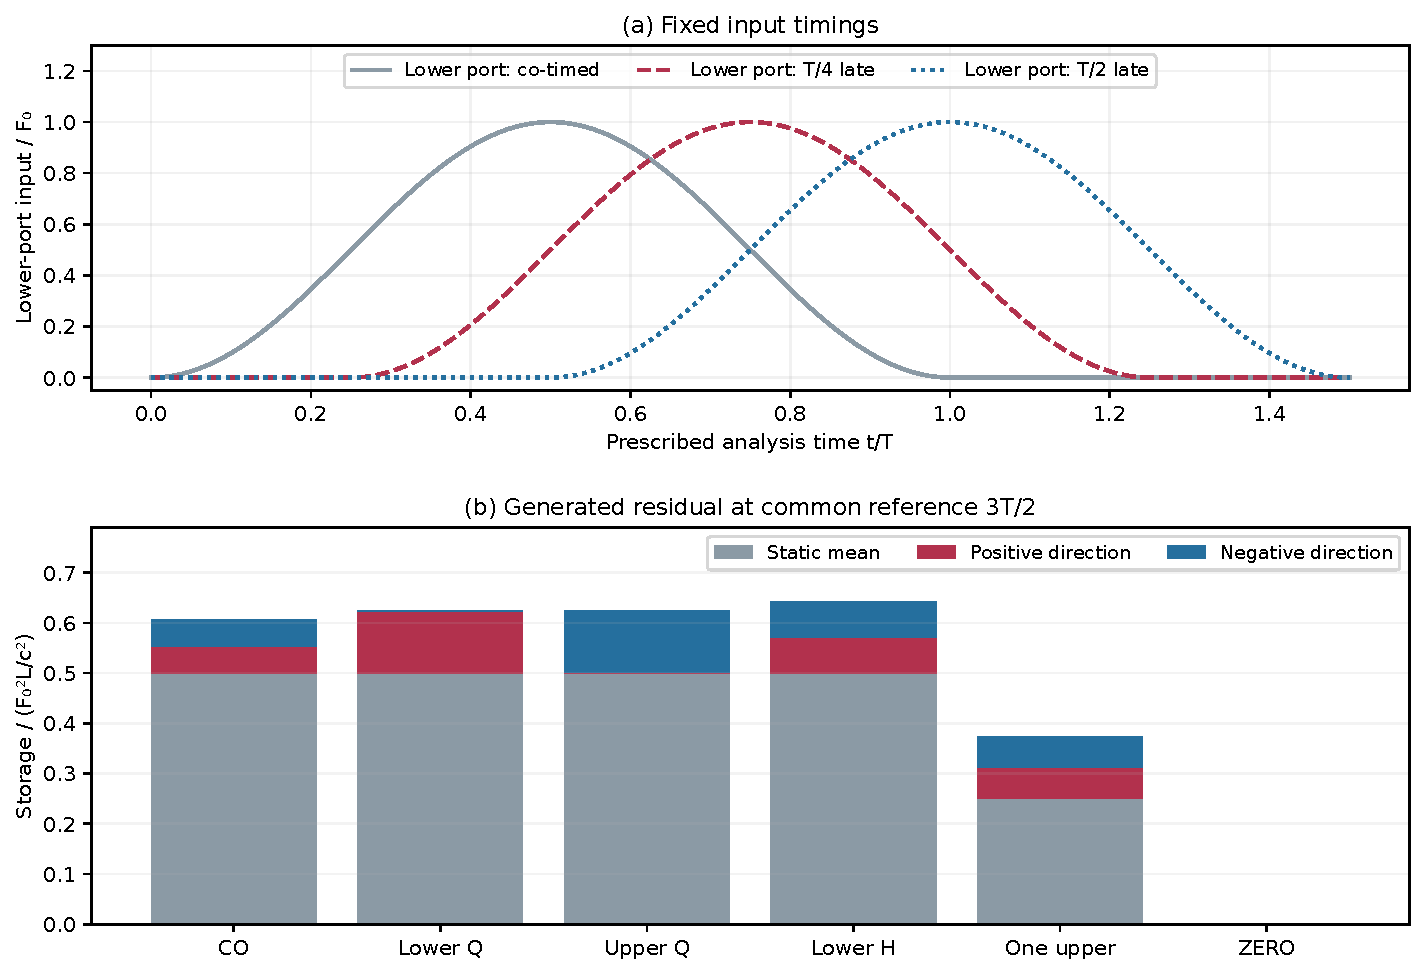
\includegraphics[width=\textwidth]{figures/timing.pdf}
\caption{Fixed prescribed delays and generated directional account, using the retained SRG-08 schedule and storage data. Every control uses the common $3T/2$ reference; no per-control rephasing or amplitude normalization is used. The weak direction of the quarter controls remains nonzero. The mean is the largest storage component.}\label{fig:timing}
\end{figure}

\subsection{Swapped timing in the actual exterior records}\label{sec:swap}
For all timing controls use the common late window
\begin{equation}\label{eq:timingwindow}
 [\tref+D_{\max}/c_e,\tref+D_{\max}/c_e+T],\qquad \tref=3T/2.
\end{equation}
Every delayed argument is at least $3T/2$, hence after the latest switch-off. In units $g_oF_0/c$, the record is
\begin{equation}\label{eq:timingrecord}
 (D_X\bar p c/F_0,0,0,0)\tr+
 \Re\left\{Q_X(\nu)\frac c{F_0}\binom{a_+}{a_-}
 e^{\ii\omega(t-3T/2)}\right\}.
\end{equation}
The amplitudes are the newly generated ones in \eqref{eq:lagamp}, not the common-envelope matrix $N$ applied outside its domain. Earlier records use the actual finite histories in \eqref{eq:composition}.

\begin{proposition}[Swapped-input distinction and its nulls]\label{prop:swap}
Equatorial scalar records of the two quarter-delay controls are identical throughout their causal histories, at every exterior speed. At $\nu=0,1$, their known-clock late scalar records differ at each retained off-height site, and their full records differ at every retained site. Scalar and total period mean-square records remain identical everywhere.
\end{proposition}
\begin{proof}
Reflection and uniqueness give $p_{\rm exchanged}(s,t)=p(L-s,t)$ and $r_{\rm exchanged}(s,t)=-r(L-s,t)$. At equatorial sites $d(s)=d(L-s)$, so reflected scalar contributions have identical delay and integrate to the same causal record. This is stronger than a late phasor collision.

Write $A=a_+$, $B=a_-$ for lower-late Q. Upper-late exchanges them. The scalar late difference is
$-2\ii g_oH(A-B)\sin\phi$. At off-height sites $\sin\phi\ne0$, $H\ne0$ by the sector theorem, and $A-B\ne0$ by \eqref{eq:quarter}, so it is nonzero. Full $Q_X$ has rank two and therefore distinguishes any distinct amplitude pairs.

For the squared records, $A,B$ have one common complex phase times real coefficients. Thus $A\overline B$ is real and unchanged by exchange. For any row $q=(q_+,q_-)$, expansion yields
\begin{equation}\label{eq:swap_power}
 |q_+A+q_-B|^2-|q_+B+q_-A|^2
 =(|A|^2-|B|^2)(|q_+|^2-|q_-|^2).
\end{equation}
The scalar column magnitudes are equal, as are the full column norms by \eqref{eq:reduction}. Their squared differences are therefore zero. The two controls have the same DC, whose cross term with a harmonic averages to zero over a period. Hence their scalar and total mean squares coincide as claimed.
\end{proof}

Individual vector components have column-square difference
$-4\Im(S_m\overline{C_m})(B\tr e_q)_j(B\tr e_\perp)_j$. It vanishes for real moments at $\nu=0$, and at equatorial sites in the fixed frames for any delay. The retained $\nu=1$ data distinguish at least one component at every fixed off-height site, with margins above their allowances. This is a finite fixture finding, not an all-position theorem or a received-energy law.

A single off-height scalar phasor distinguishes two known hypotheses but cannot invert two arbitrary complex amplitudes. With an unknown scalar clock phase, the two quarter records at one site can be made identical because they have equal magnitude and DC. A known common phase across an independent scalar stack permits a ratio inverse; independent site clocks defeat that argument. Full within-site channels retain the amplitude ratio if their nuisance factor is common. That ratio determines $\eta_{\rm osc}$, but $\eta_{\rm total}$ also needs the mean/harmonic relative calibration. A common absolute gain cancels from that relative account only if it applies to both DC and harmonic records.

For inherited matrix error $e_Q$, the phasor allowance propagates as $e_Q\norm{(a_+,a_-)}$ plus output rounding. The source record uses the old analytic truncation bound, $\sqrt8\,10^{-14}$ serialized matrix allowance, $10^{-45}$ arithmetic allowance and $10^{-14}$ output allowance. Differences add their individual bounds; stacks combine in quadrature; summaries carry $10^{-11}$. For squared magnitudes, $||z+\delta z|^2-|z|^2|\le2|z||\delta z|+|\delta z|^2$ propagates those allowances, with the period factor $1/2$. None is a formally directed-rounded enclosure. The exact scalar null and rank theorems do not rest on the numerical tables.

\section{Native readouts and a symbolic analysis-time bridge}\label{sec:native}
The pulse timings above are prescribed. They do not demonstrate that the native core supplies those histories. We now consolidate the three limited source comparisons of SRG-08, using the printed definitions in \texttt{DYNAMICS.py}, \texttt{READOUTS.py} and \texttt{Z\_MANIFOLD.py} as mathematical text.~\cite{Native,SRG08} No project function is executed. The recurrence has an integer index and no intrinsic $dt$; the supplied readout clock and carrier analysis time remain separate.

\subsection{Common finite hold and cadence aliases}
For a finite source record $f_{\pm,j}$ and symbolic $\Delta t>0$, select the common hold and end gate
\begin{equation}\label{eq:hold}
 f_\pm(t)=\sum_{j=0}^{N_s-1}f_{\pm,j}\mathbf1_{[j\Delta t,(j+1)\Delta t)}(t),
 \qquad f_\pm(t)=0\text{ outside the recorded window}.
\end{equation}
This is an interface assumption, not a native continuous-time interpolation. Its discontinuities are covered by the mild solution and integrated account.

\begin{proposition}[Hold factor and two-row determinant]\label{prop:hold}
For \eqref{eq:hold},
\begin{equation}\label{eq:holdfactor}
 \F_\pm(\omega)=H_{\Delta t}(\omega)\sum_{j=0}^{N_s-1}f_{\pm,j}e^{\ii\omega j\Delta t},
 \quad H_{\Delta t}(\omega)=e^{\ii\omega\Delta t/2}\Delta t\sinc(\omega\Delta t/2),
 \quad H_{\Delta t}(0)=\Delta t.
\end{equation}
For two rows, define
\begin{equation}\label{eq:detport}
 D_{\rm port}=f_{+,0}f_{-,1}-f_{+,1}f_{-,0}
 =-2(f_{s,0}f_{a,1}-f_{a,0}f_{s,1}).
\end{equation}
Then
\begin{equation}\label{eq:holdcriterion}
 \Im(\F_+\overline{\F_-})=-D_{\rm port}|H_{\Delta t}|^2\sin(\omega\Delta t),
 \qquad D_n=4\beta_n^2\sin(2n\theta)D_{\rm port}
 |H_{\Delta t}(\omega_n)|^2\sin(\omega_n\Delta t).
\end{equation}
\end{proposition}
\begin{proof}
Integrate $e^{\ii\omega t}$ on each hold interval after translating $t=j\Delta t+u$. The common integral on $[0,\Delta t]$ is $e^{\ii\omega\Delta t/2}\Delta t\sinc(\omega\Delta t/2)$, including its continuous value at zero. For two rows put $x=\omega\Delta t$ and expand
$(f_{+,0}+f_{+,1}e^{\ii x})(f_{-,0}+f_{-,1}e^{-\ii x})$.
Its imaginary part is $(f_{+,1}f_{-,0}-f_{+,0}f_{-,1})\sin x$. Multiplication by $|H|^2$ and substitution into \eqref{eq:criterion} prove \eqref{eq:holdcriterion}. Expanding $f_\pm=f_s\pm f_a$ proves the second expression in \eqref{eq:detport}.
\end{proof}

The discrete polynomial repeats when $\omega\Delta t$ changes by $2\pi m$; the hold factor does not generally repeat. At nonzero even multiples of $\pi$ the hold vanishes; at odd multiples its sine cross term vanishes although the hold is nonzero. The actual DC is $\Delta t\sum_j f_{\pm,j}$. For $n=1$ and nonzero determinant, the mode imbalance is nonzero exactly when $\omega_1\Delta t\notin\pi\mathbb Z$. If $\Delta t/T$ is an integer multiple of $1/2$, all eigenmode cross terms vanish at the terminal time. Other rational cadences can remove subsets of modes, with tent zeros at multiples of 32 as an additional mechanism. A nonzero first-mode term still does not prove a nonzero total signed sum for the held record.

\subsection{N0: fixed-clock macro obstruction}
\begin{proposition}[One fixed macro direction]\label{prop:N0}
At fixed clock, configuration and registration $A$, arbitrary state-norm variation of the staged $M$ readout supplies proportional real port histories. A common hold and gate preserve this property, so every $D_n$ and the total integrated flux vanish at every truncated time from zero preparation.
\end{proposition}
\begin{proof}
Equation~\eqref{eq:readouts} writes $M=zv_c$, where $v_c=(\cos\vartheta_c,\sin\vartheta_c,1)$ is fixed and $z$ is real. Fixed $A$ and the fixed normals give $f_\pm=\kappa_{\rm in}(n_\pm\tr Av_c)z$. Thus both histories are constant real multiples of one scalar history, including a possible identically zero port. Common holding and end gating multiply that same scalar record. Their finite cross transforms are real multiples of its squared magnitude, so Theorem~\ref{thm:temporal} gives zero mode-by-mode and at all truncated times.
\end{proof}
This obstruction does not require a native orbit. It is an identity of the fixed-clock readout map. Native norm variation alone cannot be promoted into two independently timed macro directions.

\subsection{N1: clock-only variation at a fixed core}
For $\Omega=(1,1,1)$ and native coefficients $k=(1,1,1)$, the radial increments $\Omega_i(k_i-|\Omega_i|^2)$ and all coupling differences vanish. The synchronization increment is a sum of sines of three times equal-phase differences and also vanishes. Thus this state is algebraically fixed, and $C=0$.

Use the admitted literal staged parameters $\lambda_{vp}=.618$, $\gamma=.577$, $\vartheta_{\rm lock}=\ell=.244$. Compare clocks
$(q,N,t_{\rm clock},q_{\rm step})=(0,12,0,1)$ and $(1,12,1/10,1)$.
With $\rho=\sqrt3/(1+\sqrt3)$ the two scalar values are
\begin{equation}\label{eq:N1z}
 z_0=.618\rho\cos(3\ell),\qquad
 z_1=.618\rho\sin(3\ell)e^{-.577/10}.
\end{equation}
Keep the already declared registration $A=aR_z(\pi/2-\ell)$. Direct rotation gives $W_r=az\cos(\vartheta_c-\ell)$ and $W_z=az$.

\begin{proposition}[Clock-only determinant]\label{prop:N1}
The two above clocks at the unchanged core give
\begin{equation}\label{eq:N1}
 \frac{D_{\rm port}}{(\kappa_{\rm in}a)^2}
 =-\frac{4\sqrt3}{7}z_0z_1\left[\cos\ell-\cos(\pi/6-\ell)\right]
 =-0.0006568730238002878\ldots<0.
\end{equation}
Repeating the same clock instead gives zero determinant.
\end{proposition}
\begin{proof}
Combine \eqref{eq:sectors} and \eqref{eq:detport} to obtain
$D_{\rm port}=-(4\sqrt3\kappa_{\rm in}^2/7)(W_{r,0}W_{z,1}-W_{z,0}W_{r,1})$.
Insert the two rotated macro vectors to get \eqref{eq:N1}. Both $z$ values are positive because $0<3\ell<\pi/2$. Also $0<\ell<\pi/12$, so $\ell<\pi/6-\ell<\pi$; cosine decreases there, making the bracket positive. The sign is therefore exact, independently of the displayed decimal. Repeated clocks yield identical vectors and zero determinant.
\end{proof}

For symbolic cadences with $\sin(\omega_1\Delta t)>0$, the first-mode bias has the negative sign of this determinant. Its origin is the readout-clock policy at unchanged $\Omega$. The exponential in \eqref{eq:N1z} belongs to the readout; it is not damping added to C1. The readout increment $1/10$ does not set $\Delta t$.

\subsection{N2: one sourced polynomial successor}
Set $\Omega_0=(1,1+\ii,2)$, $\epsilon_{\rm core}=1/20$, $g=1/5$, $k=(1,1,1)$ and phase strength zero. In that source branch, the printed recurrence is the polynomial
\begin{equation}\label{eq:nativepoly}
 \Omega_{1,i}=\Omega_{0,i}+\epsilon_{\rm core}\Omega_{0,i}(1-|\Omega_{0,i}|^2)
 +g\sum_{j\ne i}(\Omega_{0,j}-\Omega_{0,i}).
\end{equation}
There is no phase extraction or reconstruction in the zero-strength branch. We use exactly this single admitted substitution.

\begin{proposition}[One chiral compatibility witness]\label{prop:N2}
Equation~\eqref{eq:nativepoly} gives
\begin{equation}\label{eq:successor}
 \Omega_1=(6/5+\ii/5,\ 23/20+11\ii/20,\ 13/10+\ii/5),
 \quad C_0=(-2,0,1),\quad C_1=(-97/200,1/50,43/100).
\end{equation}
With the same $A=aR_z(\pi/2-\ell)$ as N1,
\begin{equation}\label{eq:N2}
 \frac{D_{\rm port}}{(\kappa_{\rm in}a)^2}
 =\frac{4\sqrt3}{7}\left(\frac38\cos\ell+\frac1{50}\sin\ell\right)
 =0.36494211036136137\ldots>0.
\end{equation}
\end{proposition}
\begin{proof}
The three coupling sums at $\Omega_0$ are $1+\ii$, $1-2\ii$, and $-2+\ii$. The radial increments are respectively $0$, $-(1+\ii)/20$ and $-3/10$. Adding these terms with their stated coefficients gives the three entries in \eqref{eq:successor}. Applying the independently defined real/imaginary cross product gives $C_0$ and $C_1$ as displayed. Under the fixed registration,
$W_r/a=\cos\ell\,C_x+\sin\ell\,C_y$ and $W_z/a=C_z$. Therefore
\[
 \frac{W_{r,0}W_{z,1}-W_{z,0}W_{r,1}}{a^2}
 =-\frac38\cos\ell-\frac1{50}\sin\ell.
\]
The determinant relation used in N1 now proves \eqref{eq:N2}. Its sign is positive since $0<\ell<\pi/2$.
\end{proof}

This is one recurrence-compatible pair, not a multi-step trajectory or a claim of typical behavior. At a cadence with positive first-mode sine it gives the opposite first-mode sign from N1, but neither example determines the signed all-mode total. Held records generally contain modes beyond $n=1$, so the retained first-harmonic $Q$ matrices apply only to an explicitly isolated first-harmonic component, not a complete native-held reception history.

The arithmetic above treats the source's decimals literally and the polynomial over exact real/complex numbers. The actual implementation uses binary64/complex128 arithmetic, with rounding, overflow and finite/nonzero intermediate restrictions in the readouts. Exact algebra is not a claim of bitwise equivalence to executing that implementation. The synchronization-zero restriction is essential. Neither the chiral definition nor these two $C$ values depend on the readout clock, and the $M$ and $C$ experiments have not been blended.

What remains for native attribution is specific: a source-defined multi-step generating/readout policy, an independently justified sample-to-analysis-time interface, and the full signed modal account. The present fixed-clock obstruction, clock-only witness and one-step compatibility witness do not supply that history or establish native circulation.

\section{Consequences and boundaries}\label{sec:conclusion}
The combined model gives a concrete answer to the paired-loop and exterior-array questions. One finite-profile, two-port input drives a single well-posed periodic state. Its signed work is determined by conjugate source responses, with a retained mean and explicit interference. The actual non-antipodal geometry controls coupling factors and resonant compatibility. It does not by itself supply a native time scale, a damping mechanism or an attracting forced state.

Position and channel choice play different roles in identification. Coplanar scalar reception has an exact reflection null: it conflates opposite travellers and the specified equal-storage shifted standing wave, and it cannot distinguish exchanged source timing throughout a causal experiment. Height supplies independent scalar phases when clocks are shared. Tangent-encoded directional channels instead provide a rank-two within-site phasor map in the proved delay range. A real snapshot or a squared record retains different information, so its conclusions cannot be substituted for the phasor theorem.

Generation matters as much as observation. The common real pulse produces standing motion and zero integrated directional bias even during forcing. General paired histories are governed by the imaginary temporal cross product, not by a verbal claim that their timings differ. A quarter-period external lag produces an impure directional residual. Its large harmonic imbalance is reduced substantially when the static mean is included. The half-period example demonstrates that terminal balance can hide an earlier nonzero integrated flux.

For the completed pulse family, the residual is exactly specified by the five real coordinates
\begin{equation}\label{eq:compact}
 (\bar p,\Re a_+,\Im a_+,\Re a_-,\Im a_-),\qquad \bar r=0.
\end{equation}
This follows directly from the absence of other residual modes and reconstructs the late records through C6. It is a sufficient representation, not a minimality, capacity or speed theorem. It does not describe the on-pulse higher-mode field, an arbitrary carrier or an arbitrary native history. The temporal features may motivate a geometric software representation, while lag aliases, calibration, interference and retention/retrieval policy remain separate questions. Computational benchmarks and nonlinear write rules belong to the subsequent computational study, not to this paper's proofs.

C1 remains an open driven comparison system. Its source-work account is not paired with a debit in the unchanged native recurrence. C6 supplies no ambient physical energy balance or receiving-load equation. These are three distinct missing interfaces: a reciprocal core exchange law, an ambient source/energy account, and receiver loading. A formal outgoing line-source wave interpretation can motivate the $1/d$ retarded kernel, but a line source may be singular on the circle and no global near-source energy or self-force construction has been supplied. Neither $E$ nor $|U|^2+\norm V^2$ is declared native physical energy. No physical experiment, quantum advantage, cognition, universal memory or autonomous circulation is established.

\subsection*{Author contribution and collaboration}
Hilmir Fr\'imann Halld\'orsson originated the geometric questions about paired regions, a transverse loop, complete surrounding modules and height/radius comparisons, and directed the research sequence. The mathematical development and manuscript preparation used iterative human--AI collaboration. The conditional laws and calibrations are identified explicitly so that geometric motivation, model adoption and proved consequence remain distinguishable. Internal model-assisted mathematical reviews informed this draft; they are not external peer review.

\appendix
\section{Reproducibility and source conventions}\label{app:repro}
The editable source uses the public-style files at the draft root, its figure PDFs, and the bibliography below. The static renderer reads copied coordinate and selected retained plot/matrix data under \texttt{data/}; it does not import a native module or integrate C1 in time. The included build guide uses an existing offline Tectonic installation and populated cache, and records the actual compiler version and notices. Font, compiler and cache binaries are not part of the review bundle.

The source-access record binds each admitted report, specification, coordinate file, response matrix and source snapshot to its supplied archive/member identity. Paper I is cited at the actual publication commit. The 18-claim ledger relates each selected claim to statement and equation labels and final PDF pages, with its source hypotheses and limits. Manuscript-local checks concern displayed identities, exact sign/reference conversions, transcribed fixed values, data provenance and label closure. Earlier suite pass counts are historical evidence and are not added to these checks.

The final page review checks all rendered pages, including proof continuations, equation breaks, captions, tables and references. Rebuilding a PDF creates a new artifact requiring its own visual review. A successful compiler exit alone is not visual QA or mathematical acceptance.

\subsection{A compact convention crosswalk}\label{app:crosswalk}
\begin{table}[htbp]\centering\small
\begin{tabular}{P{.27\textwidth}P{.29\textwidth}P{.31\textwidth}}\toprule
Source convention & Manuscript convention & Exact relationship\\\midrule
SRG-05 characteristics & $w_\sigma$ & $(p+\sigma r)/\sqrt2$\\
SRG-08 characteristics & $\widetilde w_\sigma$ & $\widetilde w_\sigma=\sqrt2w_\sigma$\\
SRG-07 residual reference & $t-T$ & $a^{[T]}$ in \eqref{eq:pulseamplitudes}\\
SRG-08 common reference & $t-3T/2$ & $a^{[3T/2]}=-a^{[T]}$ at $n=1$\\
Spatial series coefficient & $p_n$ & Coefficient of $e^{+\ii n\chi}$\\
Positive-time amplitude & $a_+$ & Coefficient inside $\Re(a_+e^{-\ii\chi}e^{+\ii\omega\tau})$\\
Exterior directional column & second column of $Q$ & $-B\tr v_-$, from the sign of $r$\\
Mean plus harmonic storage & $E_{\rm total}$ & $E_{\rm mean}+E_++E_-$\\
Integrated oriented flux & $\Jflux$ & $c(E_+-E_-)$ for one harmonic, not section power\\\bottomrule
\end{tabular}
\caption{Factors and signs retained across the four accepted source reports.}\label{tab:crosswalk}
\end{table}

\clearpage
\subsection{Information domains used in the paper}\label{app:domains}
\begin{table}[htbp]\centering\small
\begin{tabular}{P{.28\textwidth}P{.28\textwidth}P{.31\textwidth}}\toprule
Experiment & Unknowns & Required qualification\\\midrule
Forced-frequency taps & two complex port amplitudes & Nonresonant particular solution; active finite windows; independent preparation excluded\\
Free $n=1$ exterior family & two complex directional amplitudes & Known relative channels/clock; sector range for exact rank\\
One real snapshot & four real amplitude coordinates & Real matrix, not complex phasor rank; finite stack evidence separated\\
Common one-circuit pulse & two real coefficients & Known envelope; zero preparation; DC and harmonic calibrated together\\
Six fixed timing controls & six prescribed hypotheses & Shared phase origin and amplitude scale; full amplitude-family ranks are distinct\\
Native two-row hold & source-defined finite rows & Symbolic common cadence; single-mode criterion does not settle the total\\\bottomrule
\end{tabular}
\caption{The domain is part of each identifiability statement. Increasing sensor count does not change these input dimensions.}\label{tab:domains}
\end{table}

\begin{thebibliography}{9}
\bibitem{PaperI} Hilmir Fr\'imann Halld\'orsson. \emph{Paired-Gap Geometry and Toroidal Observation Maps for the Folded Tri-Octagon}. Paper I, v0.1.1, manuscript 18 October 2026; author-authorized repository edition 19 October 2026. Internally reviewed research edition. Commit \texttt{88ee0550f851507c159f4443c999b6f3ae39097d}. \href{https://github.com/pzychozen/trioctagon-physics/tree/88ee0550f851507c159f4443c999b6f3ae39097d/SRG_REDISCOVERY/PAPERS/PAIRED_GAP_GEOMETRY_OBSERVATION/publication/v0.1.1}{Commit-pinned edition and reproducible source}.
\bibitem{SRG05} Author-directed, AI-assisted SRG research record. \emph{SRG-SHARED-CARRIER-05: One Field, Two Ports, Passive Records}. Report and \emph{Conditional Carrier Specification}, 18 October 2026. Unpublished retained source; accepted within internal conditional shared-carrier scope. Sections 1--7 define the geometry, C1, account, spectrum and taps.
\bibitem{SRG06} Author-directed, AI-assisted SRG research record. \emph{SRG-EXTERIOR-OBSERVATION-06: What the Unchanged Exterior Arrays Can Distinguish}. Report, C6 specification, response matrices and quadrature record, 18 October 2026. Unpublished retained source; accepted within internal conditional exterior-observation scope. Sections 2--7 supply history bounds, symmetry, numerical qualifications and causality.
\bibitem{SRG07} Author-directed, AI-assisted SRG research record. \emph{SRG-SOURCE-TO-EXTERIOR-07: What One Paired Pulse Generates from Rest}. Report, \emph{Pulse Calibration Specification} and response data, 18 October 2026. Unpublished retained source; accepted within internal zero-prepared finite-pulse scope. Sections 2--7 supply the all-mode moments, work and generated reception.
\bibitem{SRG08} Author-directed, AI-assisted SRG research record. \emph{SRG-TEMPORAL-DIRECTIONALITY-08: When Paired Timing Creates a Directional Bias}. Report, \emph{Temporal Comparison Specification}, \emph{Native Time Convention} and response data, 18 October 2026. Unpublished retained source; accepted within internal conditional temporal-directionality scope. Sections 2--6 supply the cross-phase criterion, fixed timing controls and three native/readout comparisons.
\bibitem{Native} Tri-Octagon scientific source snapshots. \texttt{DYNAMICS.py}, \texttt{READOUTS.py}, \texttt{Z\_MANIFOLD.py}, with \texttt{FACE\_STATE.py} and \texttt{GEOMETRY.py} as geometric context. Exact text copies admitted through the SRG source chain at checkpoint \texttt{ef11dc148bea8cba6bb51e60be03fceca38cf0d4}. Retained definitions, read as text; original path and byte identities in the accompanying source map. No execution or trajectory is a source for this manuscript.
\bibitem{Reviews} \emph{SRG-05, SRG-06, SRG-07 and SRG-08 GPT Mathematical Reviews and Acceptance Records}, 18 October 2026. Retained internal model-assisted reviews. These document accepted hypotheses, exceptional cases, numerical qualifications and limited computational interpretations; they are not external peer review or physical validation.
\end{thebibliography}

\end{document}
